\chapter{绪论}
\label{cha:introduction}

\section{研究背景与意义}
\label{sec:intro}

1956,在达特茅斯会议会议上,约翰·麦卡锡等人提出了人工智能(Artificial Intelligence,AI)的概念,开辟了如今人工智能这一领域学科。当时,科学家们希望打造一台可以像人一样思考的机器,即所谓的通用人工智能。现如今,虽然我们还没有实现这个伟大的目标,但是六十年的研究与探索,在一些特定的任务上,机器已经可以取代甚至超越人类。2011年,沃森在美国智力问答节目《危险边缘》中轻松战胜了两位人类冠军,展现出人工智能在自然语言理解方面的重大突破。2016年,谷歌旗下深度思维公司研发的Alfago机器人,在围棋人机对战中,以4比1的成绩击败了世界排名第五的李世石,成为人工智能研究工作的另一个里程碑。

机器学习(Machine Learning,ML)是实现人工智能的一种有效方式。机器学习是一个涉及多个领域的交叉学科,目前并没有统一的定义。一种常见的解释是,机器学习通过模拟、归纳人类的学习行为,利用计算机强大的计算能力,让机器从大规模的数据中获取知识,不断提升机器自己的性能最终获得执行任务的能力。在机器学习多年的发展历程中,演化出诸多经典算法,例如决策树、贝叶斯分类、支持向量机、最大期望算法等。早期的这些算法均没有实现人工智能的终极目标,甚至在狭义人工智能的一些特定的任务上,也很难达到人类水平。深度学习(Deep Learning,DL)的出现,改变了这一现状。

深度神经网络(Deep Neural Network,DNN)起源于人工神经网络(Neural Networks,NN),是受生物神经科学启发演化出的计算模型。借鉴神经系统中神经元和突出连接等微观概念,最早的神经网络计算模型“感知器”(Perceptron)被提出,但是当时人工神经网络对脑科学的认知并不够深刻。深度神经网络试图通过模拟信息在大脑神经元之间的传播过程,借鉴人脑分层化的信息处理机制,一种由多层“感知器”组成的计算模型即多层感知器被提出。这种采用分层特征提取的深度神经网络,在人工智能领域取得了重大的成功。

计算机视觉(Computer Vision,CV)是人工智能领域研究热点之一,也是卷积神经网络取得巨大成功的应用领域之一。计算机视觉是一门研究如何让计算机模拟生物视觉来理解世界的科学,通过各种成像设备代替人的视觉感官,获取周围的环境信息为做系统的输入,例如通过相机获取的RGB图像、通过红外线获取的红外图像、通过热红外获取的热图等,最后通过计算机强大的计算能力来模拟人脑对环境的处理和理解,让计算机可以具有某种程度上的智能去完成一些特定的任务。


卷积神经网络(Convolutional Neural Network,CNN)促进了计算机视觉的发展与进步。受生物视觉系统启发,卷积神经网络融合了局部感受野、权值共享、池化和分层特征提取等概念。在语音识别、视觉物体识别、物体检测和基因组识别等领域,卷积神经网络均取得巨大的成功。特别是在人脸识别、自然语言处理和围棋人机对战中,卷积神经网络甚至超越了人类的水平,让我们对狭义人工智能的发展与到来,充满了信心与期待。

\section{相关研究}
\label{sec:relate}

\subsection{卷积神经网络的提出}

1943年,McCulloch等人~\cite{mcculloch1943logical}最早提出了神经网络的理论模型,当时的神经网络还不具备计算能力。1958年,康奈尔大学的Rosenblatt~\cite{rosenblatt1958perceptron}教授提出的“感知器”(Perceptron)计算模型,被认为是神经网络的始祖。据我们所知,第一个深层的神经网络是Ivakhnenko等人~\cite{ivakhnenko1966cybernetic,ivakhnenko1967cybernetics,ivakhnenko1968group,ivakhnenko1971polynomial}提出的,1971年,在其发表的重要学术论文\cite{ivakhnenko1971polynomial}中,就已经提出了一个具有八层之深的分组数据处理(Group Method of Data Handling,GMDH)多层感知器。%1975年,日本学者Fukushima提出认知机(Cognitron)~\cite{fukushima1975cognitron} 和神经认知机(Neocognitron)~\cite{fukushima1980neocognitron}模型,被认为是最早的卷积神经网络原型。

1969年,在Minsky和Papert~\cite{minsky1969perceptrons}发布的新书《感知器》中,论证了感知器存在的两个关键问题:单层的感知器无法解决复杂的非线性问题,其中提到了经典的异或操作;另外当时的计算能力也无法满足感知机的计算需求。神经网络的研究一度陷入低潮,发展缓慢,直到误差反向传播(Backpropagation,BP)算法的出现,改变了这种现象。最早的BP算法是Linnainmaa~\cite{linnainmaa1970representation,linnainmaa1976taylor}在其1970年的博士论文中提出的,当时的BP并没有用在神经网络。1973年,Dreyfus~\cite{dreyfus1973computational}将BP算法应用于最小化误差函数。据我们所知,第一个将BP应用于神经网络的算法是Werbos~\cite{werbos1982applications}于1982年提出的。但是1985年,Rumelhart和Hinton等人的论文~\cite{rumelhart1985learning}才使得神经网络的BP算法得到了广泛的关注,为神经网络的发展做出了重大的贡献。

卷积神经网络是受生物视觉皮层认知机制启发而来,1959年,Hubel和Wiesel~\cite{hubel1959receptive,hubel1962receptive}在生物视觉皮层的早期研究中,发现了在感受野范围内视觉皮层中简单细胞、复杂细胞和超复杂细胞对光信号具有不同的响应。受此启发,日本学者Fukushima于1975年提出了认知机(Cognitron)~\cite{fukushima1975cognitron} 和神经认知机(Neocognitron)~\cite{fukushima1980neocognitron}的计算模型,被认为是最早的卷积神经网络原型。1989年,LeCun等人~\cite{lecun1989backpropagation,le1990handwritten}将误差反向传播算法引入到神经认知机模型中,提出了著名的LeNet-5网络,如图~\ref{fig:lenet}所示,奠定了现代卷积神经网络的计算框架。但由于当时训练数据规模和计算机计算能力的限制,卷积神经网络并没有受到广泛的关注。直到2012年,Krizhevsky等人~\cite{krizhevsky2012imagenet}提出了一个与LeNet-5类似,但结构更深的卷积神经网络模型艾利克斯网络AlexNet,借助于高性能的GPU并行计算能力,在2012年ImageNet大规模视觉识别比赛(ImageNet Large Scale Visual Recognition Competition,ILSVRC)中一举夺冠,掀起了卷积神经网络的研究热潮。

\begin{figure*}
\centering
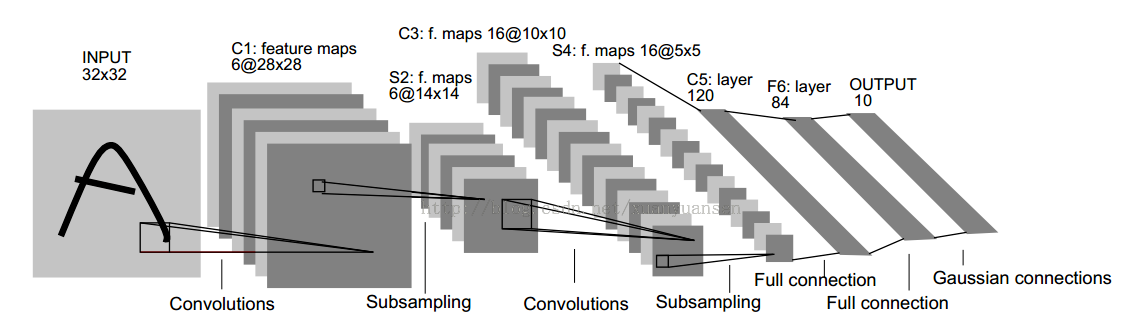
\includegraphics[width=1.0\linewidth]{intro_lenet.png}
\caption{LeNet-5~\cite{lecun1989backpropagation}网络结构。}
\label{fig:lenet}
\end{figure*}


%近年来对神经网络的研究,主要可以分为三个流派,分别是:基于概率模型的神经网络模型,基于数据或特征重构的自动编码器,和目前最受关注的卷积神经网络。

%\subsection{基于概率模型的神经网络模型}
%从概率模型观点出发,特征学习的过程可以理解为,通过对大量输入数据的观察,找到一组可以正确表示输入数据样本分布的隐层特征。对于隐层特征$h$和观测数据$x$,对$h$和$x$的联合概率分布$p(x,h)$进行建模。特征提取的过程可以看成在已知输入数据$x$的情况下,预测隐层随机变量$h$概率分布的过程,即求解后验概率分布$p(h|x)$。学习的过程可以看做是采用极大似然估计的方法,对模型参数求解的过程。概率图模型采用图结构来描述随机变量之间的依赖关系,可以分为有向概率图和无向概率图两类。它们的区别仅仅体现在联合概率的定义,但两者学习的过程和计算量却截然不同。

%有向概率图模型可以统一解释为,在已知条件概率分布$p(x|h)$和先验概率分布$p(h)$的情况下,重构联合概率$p(x,h)=p(x|h)p(h)$的过程。基于有向概率图模型的网络包括:概率主成分分析(Probabilistic Principal Component Analysis ,PPCA)~\cite{tipping1999probabilistic}、概率解释的稀疏编码~\cite{olshausen1996emergence}、Sigmoid信念网络(Sigmoid Belief Networks)~\cite{neal1992connectionist}和深度信念网络(Deep Belief Network、DBN)~\cite{hinton2006reducing}。其中概率主成分分析和概率解释的稀疏编码常常被当做深度学习发展过程中的浅层学习网络。在概率主成分分析中,假设预测数据$x$是由隐层随机变量$h$生成的,并且隐层变量$h$和条件概率$p(x|h)$均服从高斯分布:
%\begin{eqnarray} \label{equ:ppca}
%p(h)&=&\mathit{N}(h|0,\sigma_{h}^{2}\mathit{I})\nonumber\\
%p(x|h)&=&\mathit{N}(x|Wh+\mu_x,\sigma_{x}^{2}\mathit{I})
%\end{eqnarray}
%概率解释的稀疏编码与此类似,但是隐层随机变量$h$不再服从高斯分布,而是服从稀疏诱导的拉普拉斯先验(Sparsity Inducing Laplace prior):
%\begin{eqnarray} \label{equ:psc}
%p(h)&=&\prod_{i}^{d_h}exp(-{\lambda}{\lvert}h_i{\rvert})\nonumber\\
%p(x|h)&=&\mathit{N}(x|Wh+\mu_x,\sigma_{x}^{2}\mathit{I})
%\end{eqnarray}
%借鉴于视觉皮层对复杂刺激的响应方式,Olshausen指出,经稀疏编码提取的图像基函数类似于生物视觉皮层V1区简单细胞的响应特性:局限性、方向性和选择性。

%无向概率图模型,即马尔科夫随机场(Markov Random Fields,MRFs),其联合概率$p(x,h)$可以表示为:
%\begin{eqnarray} \label{equ:mrf}
%p(x,h)=\frac{1}{Z_\theta}{\prod_i\psi_i(x)}{\prod_j\eta_j(h)}{\prod_k\upsilon_k(x,h)}
%\end{eqnarray}
%其中$\psi_i(x)$,$\eta_j(h)$和$\upsilon_k(x,h)$分别表示观测数据$x$,隐随机变量$h$和它们之间相互作用的群势能(Clique Potentials);$Z_\theta$为归一化因子。玻尔兹曼机(Boltzmann)~\cite{hinton1983optimal}是MRFs的一种简化形式,可以表示:
%\begin{eqnarray} \label{equ:bz}
%p(x,h)=\frac{1}{Z_\theta}exp(-\varepsilon_\theta(x,h))
%\end{eqnarray}
%其中$\varepsilon_\theta(x,h)$是能量函数;$\theta$是模型的参数。波尔兹曼机的能量通常定义为:
%\begin{eqnarray} \label{equ:bm_e}
%\varepsilon_\theta(x,h)^{BM}=-\frac{1}{2}x^{T}Ux-\frac{1}{2}h^{T}Vh-x^{T}Wh-b^{T}x-d^{T}h
%\end{eqnarray}
%其中参数$\theta=(U,V,W,b,d)$是模型的参数,分别代表观测层对观测层、隐层对隐层、观测层对隐层、观测层自身和隐层自身的连接关系。受限波尔兹曼机(Restricted Boltzmann Machine,RBM)是对波尔兹曼机的一种简化,也是最常见得波尔兹曼机计算模型。RBM的能量函数$\varepsilon_\theta(x,h)^{RBM}$仅仅是令$\varepsilon_\theta(x,h)^{BM}$中的$U=0, V=0$。与RBM相关的研究主要集中于模型的改进与学习算法两个方向。在模型方面,包括高斯受限玻尔兹曼机(GRBM)~\cite{krizhevsky2009learning}、均值方差受限玻尔兹曼机(mcRBM)~\cite{hinton2010modeling}、mPoT模型~\cite{mnih2010generating}、钉板(Spike-and-Slab)受限玻尔兹曼机(ssRBM)~\cite{courville2011spike}和深度玻尔兹曼机(Deep Boltzmann Machine、DBM)。在学习方法上包括吉布斯采样法(Gibbs Sampling)~\cite{hinton1983optimal}、对比离差算法(Contrastive Divergence,CD)~\cite{hinton1999products,hinton2006fast}、随机最大似然法(Stochastic Maximum Likelihood、SML)~\cite{younes1999convergence}、快速持续对比离差算法(Fast-weights Persistent Contrastive Divergence,FPCD)~\cite{tieleman2009using}。
%
%
%概率模型的学习需要求隐随机变量相对于观测变量的后验概率,不论在有向图模型还是无向图模型,后验概率的计算是很复杂甚至于无法计算的,尤其是对于深层网络结构。因此通常采用采样的方法对其进行估计,这往往会引入估计误差。自动编码器(Autoencoders)~\cite{bourlard1988auto,hinton1994autoencoders}是一种直接对数据数据进行重构的特征提取方法,包括编码(encoder)和解码(decoder)两个过程,将编码和解码函数分别记为$f_\theta$和$g_\theta$,其中$\theta$是需要学习的参数。一个最基本的自动编码器可以通过最小化重构误差函数求解:
%\begin{eqnarray} \label{equ:ae}
%\mathcal{J}_{AE}(\theta)=\sum_{t}L(x^{(t)},g_{\theta}(f_{\theta}(x^{(t)})))
%\end{eqnarray}
%其中$x^{(t)}$是训练样本;$L$为L1或L2范数。与自动编码器相关的研究主要包括稀疏自动编码器(Sparse Autoencoders,SAE)~\cite{poultney2006efficient}、去噪自动编码器(Denoising Autoencoders,DAE)~\cite{vincent2008extracting}收缩自动编码器(Contractive Autoencoders,CAE)~\cite{rifai2011contractive}预测自动编码器(Predictive Sparse Decomposition,PSD)~\cite{olshausen1996emergence}等,这些方法的主要区别在于优化函数有所不同:
%\begin{eqnarray} \label{equ:aes}
%\mathcal{J}_{SAE}(\theta)&=&\sum_{t}L(x^{(t)},g_{\theta}(f_{\theta}(x^{(t)})))+\lambda\sum_{t}\lVert{h^{(t)}}\lVert_{1}\nonumber\\
%\mathcal{J}_{DAE}(\theta)&=&\sum_{t}\mathbb{E}_{q(\tilde{x}|x^{(t)})}[L(x^{(t)},g_{\theta}(f_{\theta}(x^{(t)})))]\nonumber\\
%%\mathcal{J}_{CAE}(\theta)&=&\sum_{t}L(x^{(t)},g_{\theta}(f_{\theta}(x^{(t)})))+\lambda\vert\vert{f_{\theta}(x)_j(1-f_{\theta}(x)_j)W_j}\vert\vert_{F}^{2}
%\mathcal{J}_{CAE}(\theta)&=&\sum_{t}L(x^{(t)},g_{\theta}(f_{\theta}(x^{(t)})))+\lambda\lVert{\frac{\partial{f_\theta}}{\partial{x}}(x)}\rVert_{F}^{2}\nonumber\\
%\mathcal{J}_{PSD}&=&\sum_{t}\lVert{h^{(t)}}\lVert_{1}+\lVert{x^{(t)}-Wh^{(t)}}\lVert_{2}^{2}+\lVert{h^{(t)}-f_{\alpha}(x^{(t)})}\lVert_{2}^{2}
%\end{eqnarray}


\subsection{卷积神经网络研究进展}


以LeNet-5为例,如图~\ref{fig:lenet}所示,最基本的卷积神经网络包括六个重要的组成部分~\cite{gu2015recent,bengio2013representation,bengio2009learning,lecun2010convolutional,schmidhuber2015deep,Goodfellow-et-al-2016-Book}:卷积、池化、非线性激活函数、正则化、损失函数和网络训练方法。本节按卷积神经网络的结构,对近代卷积神经网络的研究进展进行简要的综述。

卷积层是卷积神经网络最基本的组成结构,它具有局部特征提取的作用。对卷积层的改进主要体现在对卷积特征提取能力的提升,据我们了解有三种网络结构可以有效地提升卷积的特征表达能力。网络中的网络(Network in Network,NIN)~\cite{DBLP:journals/corr/LinCY13}是Lin等人在2013年提出的一种卷积层改进方法,传统的卷积层只能提取线性特征,Lin通过在传统卷积层中嵌入一个小型网络,来增强局部感受野范围内的特征表达能力与非线性,进而提升整个NIN结构的拟合能力。最大化输出单元(Maxout)~\cite{goodfellow2013maxout}是Goodfellow等人提出的,通过对多个卷积层的输出取最大输出响应,来增强卷积层的非线性拟合能力。理论上,当卷积核足够大时,具有两个隐层的Maxout可以以任意精度逼近任意连续曲线。Maxout采用线性分段函数来逼近复杂的非线性函数,的确可以提高网络的识别能力,但是需要引入大量的学习参数和计算量。Inception~\cite{szegedy2014going,szegedy2015rethinking,szegedy2016inception}是GoogLeNet的组成单元,它可以看做是对NIN的一种推广,Szegedy等人用不同大小的卷积核进行特征提取,再从多组特征中优化出表达能力最强的一组特征。

池化是卷积神经网络另一个重要概念,它将位置相邻且语义相近的一组特征规约为一个特征,通过减小特征维度来降低网络的计算复杂度,同时还可以保证特征具有一定程度的平移不变性。最常见的池化方法是均值池化(Average Pooling)和最大池化(Max Pooling)~\cite{weng1992cresceptron}。2007年,Hyvarinen等人~\cite{hyvarinen2007complex,bruna2013signal}受复杂细胞工作机制启发提出了$L_{p}$池化,通过对池化区域内的局部特征求取$p$范数来实现。均值池化和最大池化可以看成是$L_{p}$池化的两个特例,当 $p=1$ 时,$L_{p}$池化等价于均值池化;当 $p=\infty$ 时, $L_{p}$池化等价于最大池化。Yu等人~\cite{yu2014mixed}提出混合池化(Mixed Pooling)巧妙地将平均池化与最大池化进行结合,混合池化的输出响应是均值池化和最大池化的随机加权平均,随机的方式使得混合池化可以更有效地避免过拟合问题。受Dropout启发Zeiler和Fergus~\cite{zeiler2013stochastic}提出了随机池化(Stochastic Pooling)方法,根据多项式分布在池化区域内随机地选取激活值,随机池化也可以有效地避免过拟合问题。Rippel等人~\cite{rippel2015spectral}提出光谱池化(Spectral Pooling)方法,将池化操作从时域转换到频域。与最大池化相比,具有线性低通滤波的光谱池化可以有效地减少池化过程中特征的信息损失。He等人~\cite{he2014spatial}提出了金字塔池化(Spatial Pyramid Pooling,SPP)用于提取多尺度的池化特征。与全局池化~\cite{DBLP:journals/corr/LinCY13}类似,金字塔池化可以提取固定长度的特征,使网络能够直接处理不同尺度的输入图像。Gong等人~\cite{gong2014multi}提出了多尺度无序池化(Multi-scale Orderless Pooling,MOP)来增强特征的不变性。

非线性激活函数可以增强卷积神经网络的非线性拟合能力,不同的形式的激活函数,对网络的计算复杂度、特征的非线性拟合能力和网络的泛化能力具有重要的影响。线性整流单元(Rectified Linear Unit,ReLU)~\cite{nair2010rectified}是卷积神经网络最常用的激活函数,ReLU是一个分段线性函数,在保留正的激活值的同时将负的激活值抑制为零。相对于传统的Sigmoid函数与双数正切函数,ReLU的计算更加简单快速,并且可以得到稀疏的特征表达。ReLU的缺点体现在梯度反向传播的过程中,对于未激活的神经元,ReLU的反向传播梯度为零,使得未激活的神经元无法进行参数更新。针对这个问题,Mass等人~\cite{maas2013rectifier}提出斜坡线性整流单元(Leaky Rectified Linear Unit,LReLU),通过对负数部分进行线性压缩来避免零梯度的问题。He等人~\cite{he2015delving}在LReLU方法的基础上,引入可学习的参数,提出了参数化线性整流单元(Parametric Rectified Linear Unit,PReLU),将LReLU中负数部分的斜坡压缩比率从固定值转变为一个可学习的参数,PReLU通过引入极少的参数,有效地提高了网络的学习能力。对LReLU的另一项改进是Xu等人~\cite{xu2015empirical}提出的随机线性整流单元(Randomized Rectified Linear Unit,RReLU),通过均匀分布的随机随机采样来代替LReLU中固定的负数斜坡压缩比率,该方法通过引入随机变量,同样可以在一定程度上避免了过拟合问题。Clevert等人~\cite{clevert2015fast}提出指数线性单元(Exponential Linear Unit,ELU),可以在加速网络训练的同时,提高网络的识别率。相比于LReLU、PReLU和RReLU,ELU在负数部分引入了饱和机制,可以加快网络的收敛速度。此外,最大化输出单元(Maxout)~\cite{goodfellow2013maxout}和概率最大化输出单元(Probout)~\cite{springenberg2013improving}也可以看做是对激活函数的一种改进方法。

损失函数反映了估计值与真值之间的误差,不同类型的损失函数反映了对问题不同形式的定义。在多类别视觉物体识别问题中,最常用的损失函数是Softmax和多项式逻辑损失函数(Multinomial Logistic Loss)的结合形式。首先采用Softmax:${\hat{p}}_{n,k}=e^{x_n,k}/\sum_{k'=1}^{K}e^{x_{n,k'}}$ 生成 $K$ 个类别的预测概率 $({\hat{p}}_{n,1}, {\hat{p}}_{n,2}, \dots{\hat{p}}_{n,K})$,再由预测概率来计算多元逻辑回归损失。信息增益损失函数(Information Gain Loss)是多项式逻辑损失函数的一种推广,信息熵是对信息的一种量化,信息增益表示在某种特定条件下的信息熵与原信息熵的差值,信息增益损失函数常用于文本分类中,多项式逻辑损失函数可以看成是信息增益损失函数的一种特殊形式。交叉熵损失函数(Cross Entropy Loss)常被用于知识蒸馏(Distilling Knowledge)~\cite{hinton2015distilling}等相关方法,经常与Sigmoid函数配合使用,可以加快网络的收敛速度。另外一个常用的损失函数是铰链损失函数(Hinge Loss),也是支持向量机(SVM)采用的损失函数。对比损失函数(Contrastive Loss)常用于双胞胎网络(Siamese Network)~\cite{chopra2005learning},用来量化一组数据对是否属于同一类。

正则化方法可以有效地抑制过拟合现象。Dropout是Hinton等人~\cite{hinton2012improving}提出的防止网络过拟合的正则化方法,通过随机地抑制网络一部分激活值,对输出结果进行正则化。Dropout可以防止网络在分类过程中过多地依赖于一个或一小部分神经元,使网络可以在丢失一部分信息的情况下依然作出正确的预测。此外,Dropout也可以理解过一种模型平均方法。自Dropout被提出以来,出现了很多改进版本,Wang等人~\cite{wang2013fast}提出了一种快速Dropout方法,采用高斯估计来取代蒙特卡洛采样,来提高网络的训练速度。Ba等人~\cite{ba2013adaptive}提出了一种自适应Dropout方法,使隐层变量的Dropout比率可以通过一个与原网络参数共享的置信网络学习得到。Tompson等人~\cite{tompson2015efficient}发现,对 $1{\times}1$ 的卷积层进行Dropout并不能有效地防止过拟合,因此他们提出了SpatialDropout方法来解决 $1{\times}1$ 卷积层的过拟合问题。DropConnect也是受Dropout启发的一种防止网络过拟合的有效方法,与Dropout不同的是,DropConnect通过随机抑制网络的连接权来实现正则化。此外,局部响应正则化(Local Response Normalization,LRN)通过引入特征间的竞争来实现正则化的效果,通过让激活值在多个通道的局部区域相互竞争,来实现正则化的目的。批正则化(Batch Normalization,BN)~\cite{ioffe2015batch}是Ioffe等人提出的,批正则化以批为单位对特征的均值和方差进行估计,用估计的均值和方差对特征进行标准化,通过对输出特征进行约束来实现正则化的目的。


对于卷积神经网络的训练,主要涉及参数的初始化与参数更新方法两个方面。卷积神经网络具有大量的参数,一组好的初始化参数可以加快网络的收敛,Krizhevsky等人~\cite{krizhevsky2012imagenet}采用一个均值为 0 标准差为 0.01 的高斯函数对参数进行随机初始化。Glorot等人~\cite{glorot2010understanding}提出Xavier方法对高斯初始化进行了改进,依据网络输入输出神经元的个数,来调整网络参数初始化的幅度,即采用一个以 0 为均值 $2/(n_{in}+n_{out})$ 为标准差的高斯函数对网络参数进行初始化,其中 $n_{in}$ 和 $n_{out}$ 分别是输入和输出神经元的个数。He等人~\cite{he2015delving}在Xavier基础上,进一步考虑了ReLU非线性激活函数对网络参数初始化的影响,对Xavier进行改进,使改良后的Xavier适用于初始化极深的卷积神经网络,并且可以保证参数快速收敛。最常见的网络参数更新方法是随机梯度下降法(Stochastic Gradient Descent,SGD)~\cite{bottou2012stochastic},它是其他参数更新方法的基础。2011年,Duchi等人~\cite{duchi2011adaptive}提出自适应梯度法(Adaptive Gradient),通过融合梯度更新的历史信息来加快网络的收敛速度。2012年,Zeiler~\cite{zeiler2012adadelta}提出了AdaDelta方法,用于自适应地调节网络的学习率,使网络参数的更新更加鲁棒。同年,Tieleman和Hinton~\cite{tieleman2012}在Coursera公开课的讲义上提出RMSprop方法,可以自适应地更新网络的学习步长。2013年,Sutskever等人~\cite{sutskever2013importance}将NAG方法成功地应用于深层网络的训练,取得了更快的收敛速度。2015年,Kingma等人~\cite{kingma2014adam}提出了Adam方法,对动量因子进行自适应参数估计。2016年,谷歌深度思维团队提出了网络分解训练(Decoupled Neural Interfaces,DNI)~\cite{jaderberg2016decoupled},来解决网络在没有回传梯度的情况下的参数更新问题。网络分解训练通过梯度合成的方法,来预测当前层的回传梯度,打破了传统梯度下降法先前传再反传的限制,实现参数的异步更新。

%\begin{eqnarray} \label{equ:sgd}
%V_{t+1}&=&{\mu}V_t-{\alpha}{\nabla}\mathcal{L}(W_t)\nonumber\\
%W_{t+1}&=&W_t+V_{t+1}
%\end{eqnarray}
%其中 $W$ 是网络参数;$\mathcal{L}$ 是损失函数;$\alpha$ 是学习率;$\mu$ 是动量因子(Momentum)。Zeiler~\cite{zeiler2012adadelta}对SGD进行改进,使网络学习率的更新更加鲁棒,提出了AdaDelta参数更新方法:


%近年来对神经网络的研究,主要可以分为三个流派,分别是:基于概率模型的神经网络模型,基于数据或特征重构的自动编码器,和目前最受关注的卷积神经网络。


%从概率模型观点出发,特征学习的过程可以理解为,通过对大量输入数据的观察,找到一组可以正确表示输入数据样本分布的隐层特征。对于隐层特征$h$和观测数据$x$,对$h$和$x$的联合概率分布$p(x,h)$进行建模。特征提取的过程可以看成在已知输入数据$x$的情况下,预测隐层随机变量$h$概率分布的过程,即求解后验概率分布$p(h|x)$。学习的过程可以看做是采用极大似然估计的方法,对模型参数求解的过程。概率图模型采用图结构来描述随机变量之间的依赖关系,可以分为有向概率图和无向概率图两类。它们的区别仅仅体现在联合概率的定义,但两者学习的过程和计算量却截然不同。

%有向概率图模型可以统一解释为,在已知条件概率分布$p(x|h)$和先验概率分布$p(h)$的情况下,重构联合概率$p(x,h)=p(x|h)p(h)$的过程。基于有向概率图模型的网络包括:概率主成分分析(Probabilistic Principal Component Analysis ,PPCA)~\cite{tipping1999probabilistic}、概率解释的稀疏编码~\cite{olshausen1996emergence}、Sigmoid信念网络(Sigmoid Belief Networks)~\cite{neal1992connectionist}和深度信念网络(Deep Belief Network、DBN)~\cite{hinton2006reducing}。其中概率主成分分析和概率解释的稀疏编码常常被当做深度学习发展过程中的浅层学习网络。在概率主成分分析中,假设预测数据$x$是由隐层随机变量$h$生成的,并且隐层变量$h$和条件概率$p(x|h)$均服从高斯分布:
%\begin{eqnarray} \label{equ:ppca}
%p(h)&=&\mathit{N}(h|0,\sigma_{h}^{2}\mathit{I})\nonumber\\
%p(x|h)&=&\mathit{N}(x|Wh+\mu_x,\sigma_{x}^{2}\mathit{I})
%\end{eqnarray}
%概率解释的稀疏编码与此类似,但是隐层随机变量$h$不再服从高斯分布,而是服从稀疏诱导的拉普拉斯先验(Sparsity Inducing Laplace prior):
%\begin{eqnarray} \label{equ:psc}
%p(h)&=&\prod_{i}^{d_h}exp(-{\lambda}{\lvert}h_i{\rvert})\nonumber\\
%p(x|h)&=&\mathit{N}(x|Wh+\mu_x,\sigma_{x}^{2}\mathit{I})
%\end{eqnarray}
%借鉴于视觉皮层对复杂刺激的响应方式,Olshausen指出,经稀疏编码提取的图像基函数类似于生物视觉皮层V1区简单细胞的响应特性:局限性、方向性和选择性。

%无向概率图模型,即马尔科夫随机场(Markov Random Fields,MRFs),其联合概率$p(x,h)$可以表示为:
%\begin{eqnarray} \label{equ:mrf}
%p(x,h)=\frac{1}{Z_\theta}{\prod_i\psi_i(x)}{\prod_j\eta_j(h)}{\prod_k\upsilon_k(x,h)}
%\end{eqnarray}
%其中$\psi_i(x)$,$\eta_j(h)$和$\upsilon_k(x,h)$分别表示观测数据$x$,隐随机变量$h$和它们之间相互作用的群势能(Clique Potentials);$Z_\theta$为归一化因子。玻尔兹曼机(Boltzmann)~\cite{hinton1983optimal}是MRFs的一种简化形式,可以表示:
%\begin{eqnarray} \label{equ:bz}
%p(x,h)=\frac{1}{Z_\theta}exp(-\varepsilon_\theta(x,h))
%\end{eqnarray}
%其中$\varepsilon_\theta(x,h)$是能量函数;$\theta$是模型的参数。波尔兹曼机的能量通常定义为:
%\begin{eqnarray} \label{equ:bm_e}
%\varepsilon_\theta(x,h)^{BM}=-\frac{1}{2}x^{T}Ux-\frac{1}{2}h^{T}Vh-x^{T}Wh-b^{T}x-d^{T}h
%\end{eqnarray}
%其中参数$\theta=(U,V,W,b,d)$是模型的参数,分别代表观测层对观测层、隐层对隐层、观测层对隐层、观测层自身和隐层自身的连接关系。受限波尔兹曼机(Restricted Boltzmann Machine,RBM)是对波尔兹曼机的一种简化,也是最常见得波尔兹曼机计算模型。RBM的能量函数$\varepsilon_\theta(x,h)^{RBM}$仅仅是令$\varepsilon_\theta(x,h)^{BM}$中的$U=0, V=0$。与RBM相关的研究主要集中于模型的改进与学习算法两个方向。在模型方面,包括高斯受限玻尔兹曼机(GRBM)~\cite{krizhevsky2009learning}、均值方差受限玻尔兹曼机(mcRBM)~\cite{hinton2010modeling}、mPoT模型~\cite{mnih2010generating}、钉板(Spike-and-Slab)受限玻尔兹曼机(ssRBM)~\cite{courville2011spike}和深度玻尔兹曼机(Deep Boltzmann Machine、DBM)。在学习方法上包括吉布斯采样法(Gibbs Sampling)~\cite{hinton1983optimal}、对比离差算法(Contrastive Divergence,CD)~\cite{hinton1999products,hinton2006fast}、随机最大似然法(Stochastic Maximum Likelihood、SML)~\cite{younes1999convergence}、快速持续对比离差算法(Fast-weights Persistent Contrastive Divergence,FPCD)~\cite{tieleman2009using}。
%
%
%概率模型的学习需要求隐随机变量相对于观测变量的后验概率,不论在有向图模型还是无向图模型,后验概率的计算是很复杂甚至于无法计算的,尤其是对于深层网络结构。因此通常采用采样的方法对其进行估计,这往往会引入估计误差。自动编码器(Autoencoders)~\cite{bourlard1988auto,hinton1994autoencoders}是一种直接对数据数据进行重构的特征提取方法,包括编码(encoder)和解码(decoder)两个过程,将编码和解码函数分别记为$f_\theta$和$g_\theta$,其中$\theta$是需要学习的参数。一个最基本的自动编码器可以通过最小化重构误差函数求解:
%\begin{eqnarray} \label{equ:ae}
%\mathcal{J}_{AE}(\theta)=\sum_{t}L(x^{(t)},g_{\theta}(f_{\theta}(x^{(t)})))
%\end{eqnarray}
%其中$x^{(t)}$是训练样本;$L$为L1或L2范数。与自动编码器相关的研究主要包括稀疏自动编码器(Sparse Autoencoders,SAE)~\cite{poultney2006efficient}、去噪自动编码器(Denoising Autoencoders,DAE)~\cite{vincent2008extracting}收缩自动编码器(Contractive Autoencoders,CAE)~\cite{rifai2011contractive}预测自动编码器(Predictive Sparse Decomposition,PSD)~\cite{olshausen1996emergence}等,这些方法的主要区别在于优化函数有所不同:
%\begin{eqnarray} \label{equ:aes}
%\mathcal{J}_{SAE}(\theta)&=&\sum_{t}L(x^{(t)},g_{\theta}(f_{\theta}(x^{(t)})))+\lambda\sum_{t}\lVert{h^{(t)}}\lVert_{1}\nonumber\\
%\mathcal{J}_{DAE}(\theta)&=&\sum_{t}\mathbb{E}_{q(\tilde{x}|x^{(t)})}[L(x^{(t)},g_{\theta}(f_{\theta}(x^{(t)})))]\nonumber\\
%%\mathcal{J}_{CAE}(\theta)&=&\sum_{t}L(x^{(t)},g_{\theta}(f_{\theta}(x^{(t)})))+\lambda\vert\vert{f_{\theta}(x)_j(1-f_{\theta}(x)_j)W_j}\vert\vert_{F}^{2}
%\mathcal{J}_{CAE}(\theta)&=&\sum_{t}L(x^{(t)},g_{\theta}(f_{\theta}(x^{(t)})))+\lambda\lVert{\frac{\partial{f_\theta}}{\partial{x}}(x)}\rVert_{F}^{2}\nonumber\\
%\mathcal{J}_{PSD}&=&\sum_{t}\lVert{h^{(t)}}\lVert_{1}+\lVert{x^{(t)}-Wh^{(t)}}\lVert_{2}^{2}+\lVert{h^{(t)}-f_{\alpha}(x^{(t)})}\lVert_{2}^{2}
%\end{eqnarray}
%
%
%深度学习的另外一个分支卷积神经网络是受生物视觉皮层认知机制启发而来。1959年,Hubel和Wiesel~\cite{hubel1959receptive,hubel1962receptive}在生物视觉皮层的早期研究中,发现了在感受野范围内视觉皮层中简单细胞、复杂细胞和超复杂细胞对光信号具有不同的响应。受此启发,日本学者Fukushima提出了认知机(Cognitron)~\cite{fukushima1975cognitron} 和神经认知机(Neocognitron)~\cite{fukushima1980neocognitron}的计算模型,通常被认识是最早卷积神经网络模型。1989年,LeCun等人~\cite{lecun1989backpropagation,le1990handwritten}将误差反向传播算法引入到神经认知机模型中,提出了著名的LeNet-5网络,如图~\ref{fig:lenet}所示,奠定了现代卷积神经网络的计算框架。但由于当时训练数据规模和计算性能上的限制,卷积神经网络并没有受到广泛的关注。
%
%2012年,Krizhevsky等人~\cite{krizhevsky2012imagenet}提出了一个与LeNet-5类似,但结构更深的卷积神经网络模型AlexNet,借助于高性能的GPU并行计算能力,在2012年ImageNet大规模视觉识别比赛(ImageNet Large Scale Visual Recognition Competition,ILSVRC)中一举夺冠,掀起了卷积神经网络的研究热潮。此后,各种网络模型如ZFNet~\cite{zeiler2014visualizing},VGGNet~\cite{simonyan2014very},GoogleNet~\cite{szegedy2014going,szegedy2015rethinking,szegedy2016inception}、ResNet~\cite{he2015deep}等被相继提出,用以解决计算机视觉问题。



%
%\begin{figure*}
%\centering
%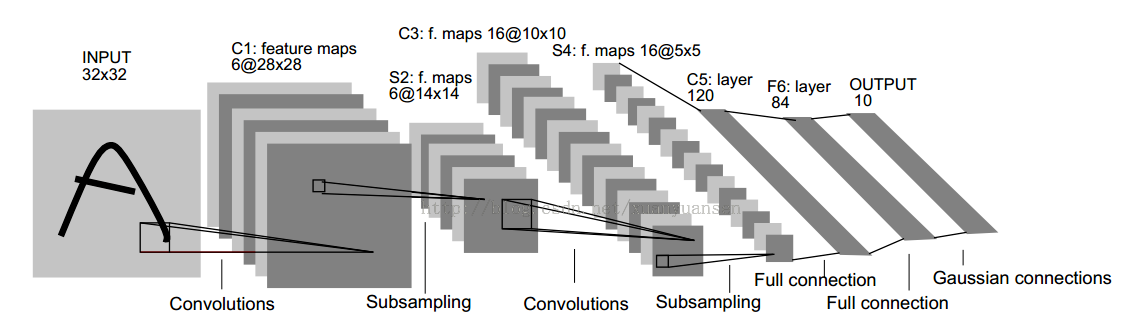
\includegraphics[width=1.0\linewidth]{intro_lenet.png}
%\caption{LeNet-5~\cite{lecun1989backpropagation}网络结构。}
%\label{fig:lenet}
%\end{figure*}
%
%以LeNet-5为例如图~\ref{fig:lenet}所示,最基本的卷积神经网络包括六个重要的组成部分~\cite{gu2015recent}:卷积、池化、非线性激活函数、正则化、损失函数和网络训练。下面我们将分别介绍卷积神经网络各部分的改进。
%
%卷积层是卷积神经网络最基本的组成结构,主要用于特征提取。对卷积层的改进主要体现在对特征提取能力的增强,据我们了解有三种网络结构可以有效的提升特征表达能力。网络中的网络(Network in Network,NIN)~\cite{DBLP:journals/corr/LinCY13}是Lin等人提出的,传统的卷积层只能提取线性特征,Lin通过在传统卷积层中嵌入一个小型网络来特征卷积层的逼近能力。最大输出单元(Maxout)~\cite{goodfellow2013maxout}是Goodfellow等人提出的,通过对多个卷积层的输出求最大的方式,来增强卷积层的拟合能力。理论上,当卷积核足够大时两个隐层的Maxout可以以任意精度逼近任意曲线。Inception~\cite{szegedy2014going,szegedy2015rethinking,szegedy2016inception}可以看做是对NIN的推广,Szegedy等人用不同大小的卷积核提取出不同形式的特征,再从中优化出表达能力最强的一组特征。
%
%池化是卷积神经网络的一个重要概念,它可以通过减小特征维度从而降低网络的计算量,同时可以使得特征具有一定的平移不变性。最长见的池化方法是均值池化(Average Pooling)和最大池化(Max Pooling)~\cite{weng1992cresceptron}。$L_{p}$池化~\cite{hyvarinen2007complex,bruna2013signal}是受复杂细胞工作机制启发的一种池化方法,$L_{p}$池化可以表示为:
%\begin{eqnarray} \label{equ:lp}
%h_{i,j,k}=[\sum_{(m,n)\in{\mathcal{R}_{ij}}}(x_{m,n,k})^p]^{1/p}
%\end{eqnarray}
%其中 $h_{i,j,k}$ 表示第 $k$ 个通道上位置 $(i,j)$ 处池化输出;$x_{m,n,k}$ 表示 $(m,n)\in\mathcal{R}_{i,j}$ 位置上特征值;$\mathcal{R}_{i,j}$代表位置 $(i,j)$ 的池化区域。当 $p=1$ 时,$L_{p}$池化等价于均值池化;当 $p=\infty$ 时, $L_{p}$池化等价于最大池化。Yu等人~\cite{yu2014mixed}采用混合池化(Mixed Pooling)巧妙地将平均池化与最大池化有效结合,混合池化可以表示为:
%\begin{eqnarray} \label{equ:mp}
%h_{i,j,k}={\lambda}{\max_{(m,n)\in\mathcal{R}_{i,j}}x_{m,n,k}}+(1-\lambda)\frac{1}{|\mathcal{R}_{i,j}|}{\sum_{(m,n)\in\mathcal{R}_{i,j}}x_{m,n,k}}
%\end{eqnarray}
%其中 $\lambda$ 是一个在 0 或 1 之间取值的随机数。受Dropout启发Zeiler和Fergus~\cite{zeiler2013stochastic}提出了随机池化(Stochastic pooling)方法,可以通过随机操作防止过拟合。Rippel等人~\cite{rippel2015spectral}提出光谱池化(Spectral Pooling)方法,通过将卷积操作从时域转换到频域,可以有效地减少池化过程中特征信息损失的问题。He等人~\cite{he2014spatial}提出了金字塔池化(Spatial Pyramid Pooling,SPP)用于提出固定长度的特征,是对~\cite{DBLP:journals/corr/LinCY13}中全局池化的一种推广。Gong等人~\cite{gong2014multi}提出了多尺度无序池化(Multi-scale Orderless Pooling ,MOP)来增强特征的不变形。
%
%非线性激活函数可以增强卷积神经网络的非线性拟合能力,不同的激活函数形式,对网络的计算量、拟合和泛化能力具有重要的影响。线性整流单元(Rectified linear unit,ReLU)~\cite{nair2010rectified}是目前卷积神经网络最常用的激活函数,ReLU可以表示为:
%\begin{eqnarray} \label{equ:relu}
%h_{i,j,k}=\max(x_{i,j,k},0)
%\end{eqnarray}
%其中$x_{i,j,k}$表示第 $k$ 个通道位置 $(i,j)$ 处的输入特征。相对于传统的Sigmoid函数:
%\begin{eqnarray} \label{equ:sigmoid}
%h_{i,j,k}=\frac{1}{1+e^{-x_{i,j,k}}}
%\end{eqnarray}
%和双曲正切函数:
%\begin{eqnarray} \label{equ:tanh}
%h_{i,j,k}=\frac{e^{x_{i,j,k}}-e^{-x_{i,j,k}}}{e^{x_{i,j,k}}+e^{-x_{i,j,k}}}
%\end{eqnarray}
%ReLU的计算更简单,并且可以得到稀疏的特征表示。但是对于未激活的神经元,ReLU的反向传播梯度为0,使得未激活的神经元无法进行参数更新。Mass等人~\cite{maas2013rectifier}提出斜坡线性整流单元(Leaky Rectified linear unit,LReLU)来解决这个问题,计算公式如下:
%\begin{eqnarray} \label{equ:lrelu}
%h_{i,j,k}=\max(x_{i,j,k},0)+{\lambda}\min(x_{i,j,k},0)
%\end{eqnarray}
%其中$\lambda$是一个预定义的取值在 $(0,1)$ 之间的随机变量。He等人~\cite{he2015delving}对LReLU进一步改进,提出了参数化线性整流单元(Parametric Rectified linear unit,PReLU),PReLU可以表示为:
%\begin{eqnarray} \label{equ:prelu}
%h_{i,j,k}=\max(x_{i,j,k},0)+{\lambda}_k\min(x_{i,j,k},0)
%\end{eqnarray}
%其中 ${\lambda}_k$ 是第 $k$ 个通道上的可学习参数。PReLU通过引入极少的参数,有效地提高了网络的拟合能力。对LReLU的另一项改进是Xu等人~\cite{xu2015empirical}提出的随机线性整流单元(Randomized Rectified linear unit,ReLU),与公式~\ref{equ:prelu}具有相同的形式,但是其中的 ${\lambda}_k$ 服从均匀分布,前向传播过程中通过随机采样产生。Clevert等人~\cite{clevert2015fast}提出了指数线性单元(Exponential Linear Unit,ELU),可以在加速网络的训练的同时,提高网络的识别率,ELU可以表示为:
%\begin{eqnarray} \label{equ:elu}
%h_{i,j,k}=\max(x_{i,j,k},0)+\min({\lambda}(e^{z_{i,j,k}}-1),0)
%\end{eqnarray}
%其中 $\lambda$ 是一个预定义的加权因子。
%
%损失函数反映了估计值与真值之间的误差,不同类型的损失函数反映了对问题的不同定义。在多类别物体分类问题中,最常用的损失函数是Softmax和多项式逻辑损失函数(Multinomial Logistic Loss)结合的一种形式。首先采用Softmax:${\hat{p}}_{n,k}=e^{x_n,k}/\sum_{k'=1}^{K}e^{x_{n,k'}}$生成 $K$ 个类别上的预测概率 $({\hat{p}}_{n,1}, {\hat{p}}_{n,2}, \dots{\hat{p}}_{n,K})$,再通过预测概率计算多元逻辑回归损失:
%\begin{eqnarray} \label{equ:softmax}
%\mathcal{L}=-\frac{1}{N}[\sum_{n=1}^{N}\sum_{k=1}^{K}\delta\{l_{n}=k\}log{\hat{p}}_{n,k}]
%\end{eqnarray}
%其中 $N$ 代表样本总数;$l$ 是样本的正确标签,$\delta$ 是指示器函数。信息增益损失函数(Information Gain Loss)是多项式逻辑损失函数的一种推广,信息熵是对信息的一种量化,信息增益表示在某种特定条件下的信息熵与原信息熵的差值,信息增益损失函数常用于文本分类中,可以公式化描述为:
%\begin{eqnarray} \label{equ:information}
%\mathcal{L}=-\frac{1}{N}\sum_{n=1}^{N}\sum_{k=1}^{K}H_{l_n,k}log({\hat{p}}_{n,k})
%\end{eqnarray}
%其中 $H$ 是信息增益矩阵,当 $H=I$时,信息增益损失函数等价于多项式逻辑损失函数。交叉熵损失函数(Cross Entropy Loss)常被用于知识蒸馏(Distilling Knowledge)~\cite{hinton2015distilling}等相关方法中,经常与Sigmoid函数配合使用,加快网络的训练速度,交叉熵损失函数定义为:
%\begin{eqnarray} \label{equ:cross}
%\mathcal{L}=\frac{1}{N}\sum_{n=1}^{N}[p_n log{\hat{p}}_n+(1-p_n)log(1-{\hat{p}}_n)]
%\end{eqnarray}
%另外一个常用的损失函数是铰链损失函数(Hinge Loss),也是支持向量机(SVM)中采用的损失函数,定义为:
%\begin{eqnarray} \label{equ:hinge}
%\mathcal{L}=\frac{1}{N}\sum_{n=1}^{N}\sum_{k=1}^{K}[max(0,1-\delta\{l_n=k\}W^{T}x_{n})]^p
%\end{eqnarray}
%其中 $W$ 是分类器线性权重矩阵,$\delta$ 是一个映射到 $[-1,1]$ 的指示器函数;$p=1$ 表示 $L_1$ 范数,$p=2$ 表示 $L_2$ 范数。对比损失函数(Contrastive Loss)常用于双胞胎网络(Siamese Network)~\cite{chopra2005learning},用来量化一组数据对是否属于同一类,定义为:
%\begin{eqnarray} \label{equ:contrastive}
%\mathcal{L}=\frac{1}{2N}\sum_{n=1}^{N}\delta(l_n^{(a)}=l_n^{(b)})d^2+\delta(l_n^{(a)}\not{=}l_n^{(b)})max(margin-d,0)^2
%\end{eqnarray}
%其中 $d=||x_n^{(a)}-x_n^{(b)}||_2$ 代表 $a$ 和 $b$ 两个网络特征向量 $x_n$ 的欧氏距离。
%
%
%正则化方法可以有效地抑制过拟合现象。Dropout是Hinton等人~\cite{hinton2012improving}首次提出的防止网络过拟合的方法,通过随机地抑制网络一部分激活值,对输出结果进行正则化。此外,Dropout也可以理解过一种模型平均技术。自Dropout提出以来,出现了很多改进版本,例如快速Dropout方法~\cite{wang2013fast}、自适应Dropout方法~\cite{ba2013adaptive}和空间Dropout方法~\cite{tompson2015efficient}。DropConnect也是受Dropout启发的一种防止网络过拟合的有效方法,与Dropout不同的是,DropConnect通过随机抑制网络的连接权来实现正则化。局部响应正则化(Local Response Normalization,LRN)通过引入特征间的竞争来实现正则化的效果,LRN可以表示为:
%\begin{eqnarray} \label{equ:lrn}
%h_{i,j,k}=x_{i,j,k}/(k+{\alpha}\sum_{l=max(0,i-n/2)}^{min(N-1,i+n/2)}(x_{i,j,l})^{2})^{\beta}
%\end{eqnarray}
%其中$k,n,\alpha,\beta$是规则化的超参,通过让激活值在 $n$ 个通道内竞争,来实现正则化的目的。批正则化(Batch Normalization,BN)~\cite{ioffe2015batch}是Ioffe等人提出,通过对输出数据进行约束来实现正则化的目的,可以表示为:
%\begin{eqnarray} \label{equ:bn}
%\hat{x}_{i,j,k}&=&(x_{i,j,k}-\mu_{k})/\sqrt{(\delta_{k}^{2}+\epsilon)}\nonumber\\
%h_{i,j,k} &=& BN(x_{i,j,k}) = \gamma\hat{x}_{i,j,k}+\beta
%\end{eqnarray}
%其中 $\mu_{k}$ 和 $\delta_{k}$ 是每批养样本在通道 $k$ 上的均值与方差;$\gamma$ 和 $\beta$ 是可学习的参数,用于增强BN的特征表达能力。
%
%对于卷积神经网络的训练,主要涉及参数的初始化与更新方法。卷积神经网络具有大量的参数,一组好的初始化参数可以加快网络的收敛,Krizhevsky等人~\cite{krizhevsky2012imagenet}采用一个均值为 0 标准差为 0.01 的高斯函数对参数进行随机初始化。Glorot等人~\cite{glorot2010understanding}提出Xavier方法对高斯初始化进行了改进,通过网络输入输出神经元的个数,来调整网络参数初始化的幅度,即采用一个以 0 为均值 $2/(n_{in}+n_{out})$ 为标准差的高斯函数对网络参数进行初始化,其中 $n_{in}$ 和 $n_{out}$ 分别是输入和输出神经元的个数。He等人~\cite{he2015delving}在Xavier基础上,进一步考虑了ReLU非线性激活函数对网络参数初始化的影响,对Xavier进行改进,使其适用于初始化极深的卷积神经网络并可以快速收敛。最常见的网络参数更新方法是梯度下降法(Stochastic Gradient Descent,SGD)~\cite{bottou2012stochastic},可以表示为:
%\begin{eqnarray} \label{equ:sgd}
%V_{t+1}&=&{\mu}V_t-{\alpha}{\nabla}\mathcal{L}(W_t)\nonumber\\
%W_{t+1}&=&W_t+V_{t+1}
%\end{eqnarray}
%其中 $W$ 是网络参数;$\mathcal{L}$ 是损失函数;$\alpha$ 是学习率;$\mu$ 是动量因子(Momentum)。Zeiler~\cite{zeiler2012adadelta}对SGD进行改进,使网络学习率的更新更加鲁棒,提出了AdaDelta参数更新方法:
%\begin{eqnarray} \label{equ:sgd}
%(v_t)_i&=&\frac{RMS((v_{t-1})_i)}{RMS(\nabla\mathcal{L}(W_t))_i}(\nabla\mathcal{L}(W_t))_i\nonumber\\
%RMS(\nabla\mathcal{L}(W_t))_i&=&\sqrt{E[g^2]+\epsilon}\nonumber\\
%E[g^2]_t&=&{\delta}E[g^2]_{t-1}+(1-\delta)g_{t}^2\nonumber\\
%(W_{t+1})_i&=&(W_t)_i-\alpha(v_t)_i
%\end{eqnarray}
%此外,自适应梯度法(Adaptive Gradient)~\cite{duchi2011adaptive}、Adam法~\cite{kingma2014adam}、Nesterov梯度法~\cite{sutskever2013importance}、RMSProp等都是基于梯度下降的改进方法。2016年,谷歌DeepMind提出了网络分解训练(Decoupled Neural Interfaces,DNI)~\cite{jaderberg2016decoupled},来解决在网络没有回传梯度的情况下,参数的更新问题。网络分解训练通过梯度合成的方法,来预测当前层的梯度,打破了传统梯度下降法先前传再反传的限制,实现参数的异步更新。
%
%此外,卷积神经网络在语音识别(Speech Recognition)、信号处理(Signal Processing)、物体检测与识别(Object Detection and Recognition)、文本的检测与识别(Text Detection and Recognition)、多任务迁移学习(Multitask and Transfer Learning)等诸多领域都取得了重大的创新与突破。

\section{预备知识}

卷积神经网络是一种特殊的神经网络结构,它采用卷积操作代替了传统神经网络的矩阵乘法操作。本节介绍卷积神经网络相关的预备知识,主要包括卷积神经网络的卷积操作、卷积操作的动机与优势、池化和非线性化。

\begin{figure}[h]
\centering
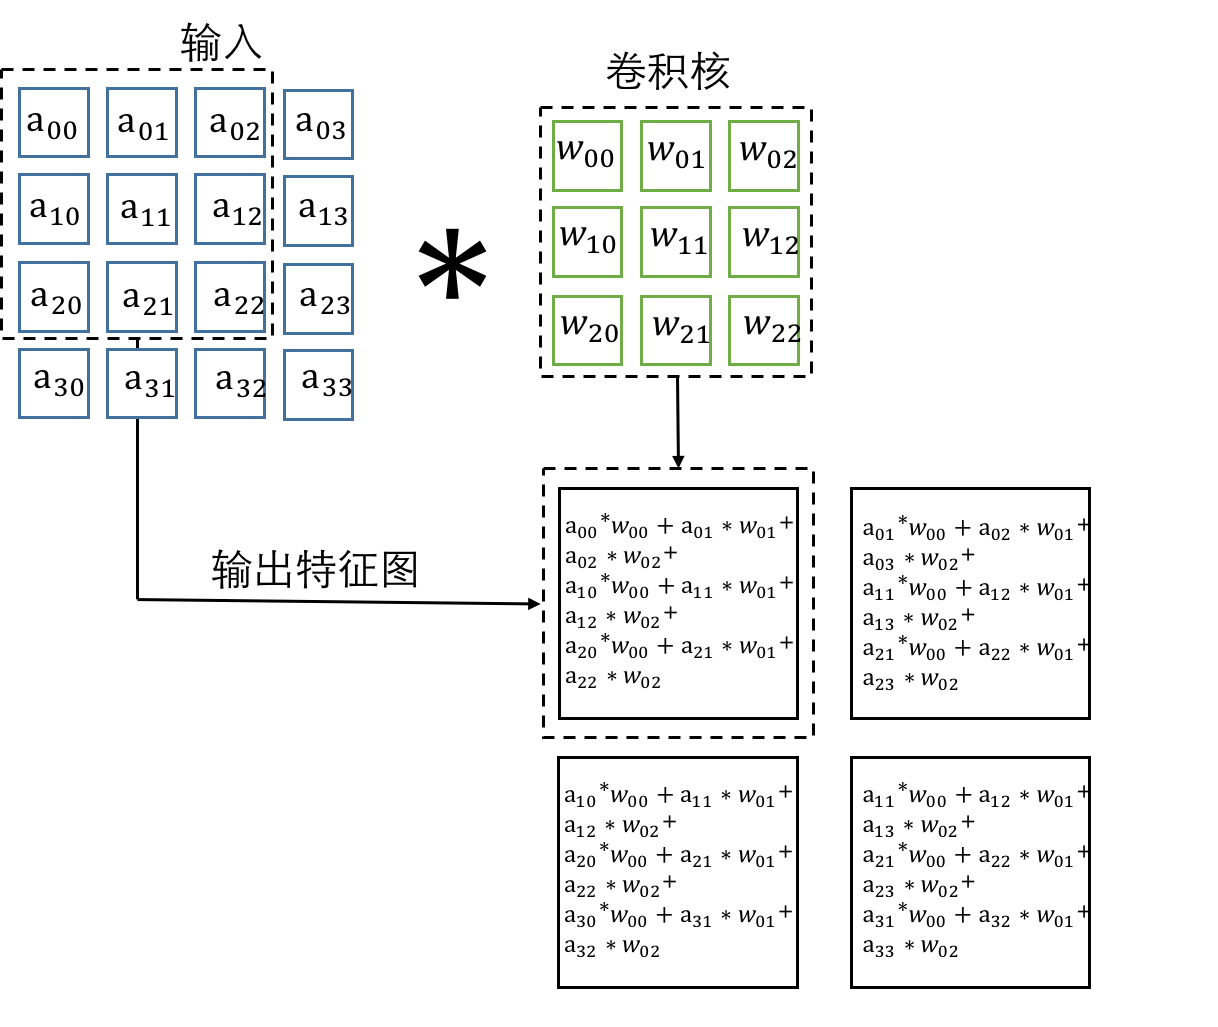
\includegraphics[width=1\linewidth]{intro_conv.png}
\caption{卷积神经网络中卷积操作实现方式。传统的卷积操作需要对卷积核进行反转,使卷积具有交换律。在卷积神经网络中,交换律并不重要,卷积网络通过端到端学习的方式,可以学习到一组位置相关的卷积核参数,是否对卷积核进行反转不会影响卷积的输出结果。本文沿用了大多数卷积神经网络库函数中卷积操作的实现方式。}
\label{fig:intro_conv}
\end{figure}

为了引出卷积神经网络中卷积操作的定义,我们首先分析在最一般的形式中,两个函数的卷积操作定义。假设我们正在使用一个雷达设备对一个物体进行跟踪,雷达设备给出了一个输出序列 $x(t)$,表示物体在 $t$ 时刻的位置。这里 $x$ 和 $t$ 都是实数,在不同的时刻 $t$ 我们可以得到一个不同的观测位置 $x(t)$。因为雷达的输出具有噪声,为了较小噪声对物体测距的影响,我们希望通过多次测量求均值的方式来减弱噪声影响。当然,当前时刻的观测值与物体的真实位置最为相关,因此我们希望在加权平均的过程中,对当前时刻的观测值赋予更高的权重。通过使用一个加权函数 $w(t)$ 来实现这样的目的,其中 $t$ 代表观测量的有效时间。每一个时刻我们均采用这用加权平均的方式对观测物体的位置进行平滑,则得到一个新的函数 $s(t)$ ,表示 $t$ 时刻平滑后的观测物体位置,如公式(~\ref{equ:convolution1})所示:
\begin{eqnarray} \label{equ:convolution1}
s(t)=\int{x(a)w(t-a)da}
\end{eqnarray}
这个操作即为两个函数的卷积操作,卷积通常可以记为星号乘法运算:
\begin{eqnarray} \label{equ:convolution2}
s(t)=(x*w)(t)
\end{eqnarray}
在上述例子中,$w$ 是一个概率密度函数,并且对于负的时间序列,$w$ 需要置为零。实际上,这些限制仅仅针对于上述雷达测距的例子,通常来讲,卷积可以定义在满足公式 (\ref{equ:convolution1})的任意函数上,可以用来表示除加权平均之外的其他含义。在上述例子中,我们假设雷达的观测是一个与时间相关的连续函数,但是计算机可以处理的数据往往是离散的。如果我们假设 $x(t)$ 和 $w(t)$ 是定义在正整数集合 $t$ 上的离散函数,上述卷积操作可以表示为:
\begin{eqnarray} \label{equ:convolution3}
s(t)=(x*w)(t)=\sum_{a=-\infty}^{\infty}x(a)w(t-a)
\end{eqnarray}

在卷积神经网络中,上述例子中的 $x$ 通常表示输入,函数 $w$ 表示特征核,输出 $s$ 称为特征图。卷积神经网络的输入、特征核和输出特征图均是多维矩阵,对于输入是二维图像的情况下,卷积操作可以表示为:
\begin{eqnarray} \label{equ:c1}
s(i,j)=(I*K)(i,j)=\sum_{m}\sum_{n}I(m,n)K(i-m,j-n)
\end{eqnarray}
卷积操作满足交换律,因此我们可以将图像的卷积表示成一种更为直观的方式:
\begin{eqnarray} \label{equ:c2}
s(i,j)=(I*K)(i,j)=\sum_{m}\sum_{n}I(i-m,j-n)K(m,n)
\end{eqnarray}

卷积操作满足交换律是因为我们对卷积核进行了反转,公式(\ref{equ:c1})中,随着 $m$ 的增大,输入图像的索引随之增大,但是卷积核的索引随之减小。但是这样的性质在卷积神经网络并不是必要的,因此在很多卷积神经网络相关的库函数中,采用一种与图像卷积相似但不具有特征核反转的卷积操作:
\begin{eqnarray} \label{equ:c3}
s(i,j)=(I*K)(i,j)=\int_{m}\int_{n}I(i+m,j+n)K(m,n)
\end{eqnarray}


在很多机器学习相关的库函数中,均采用公式(\ref{equ:c3})的卷积实现方式,本文我们沿用这样的表示方法。实际上,是否对卷积核进行反转对卷积的结果并没有太大的影响,卷积神经网络端到端的训练方法,可以使网络学习到一组位置相关的卷积核参数。图~\ref{fig:intro_conv} 是公式(\ref{equ:c3})所描述的一个卷积操作示例,对于输入为 $4\times4$ 像素大小的输入图像,采用 $3\times3$ 感受野大小的卷积核对其进行卷积,在步长为 1 且没有边界扩展的情况下,输出了一个 $2\times2$ 像素大小的特征图,特征图中每个位置的计算过程如图~\ref{fig:intro_conv} 所示。

图像卷积利用了三个重要思想来提高卷积的特征表达能力:稀疏表达、权值共享和平移同变性。此外,卷积神经网络采用卷积堆叠的方式来实现更大范围感受野的特征提取,从而实现不同规模输入图像的特征提取。下面我们将分别介绍卷积操作的这三个重要特点。


\begin{figure}[h]
\centering
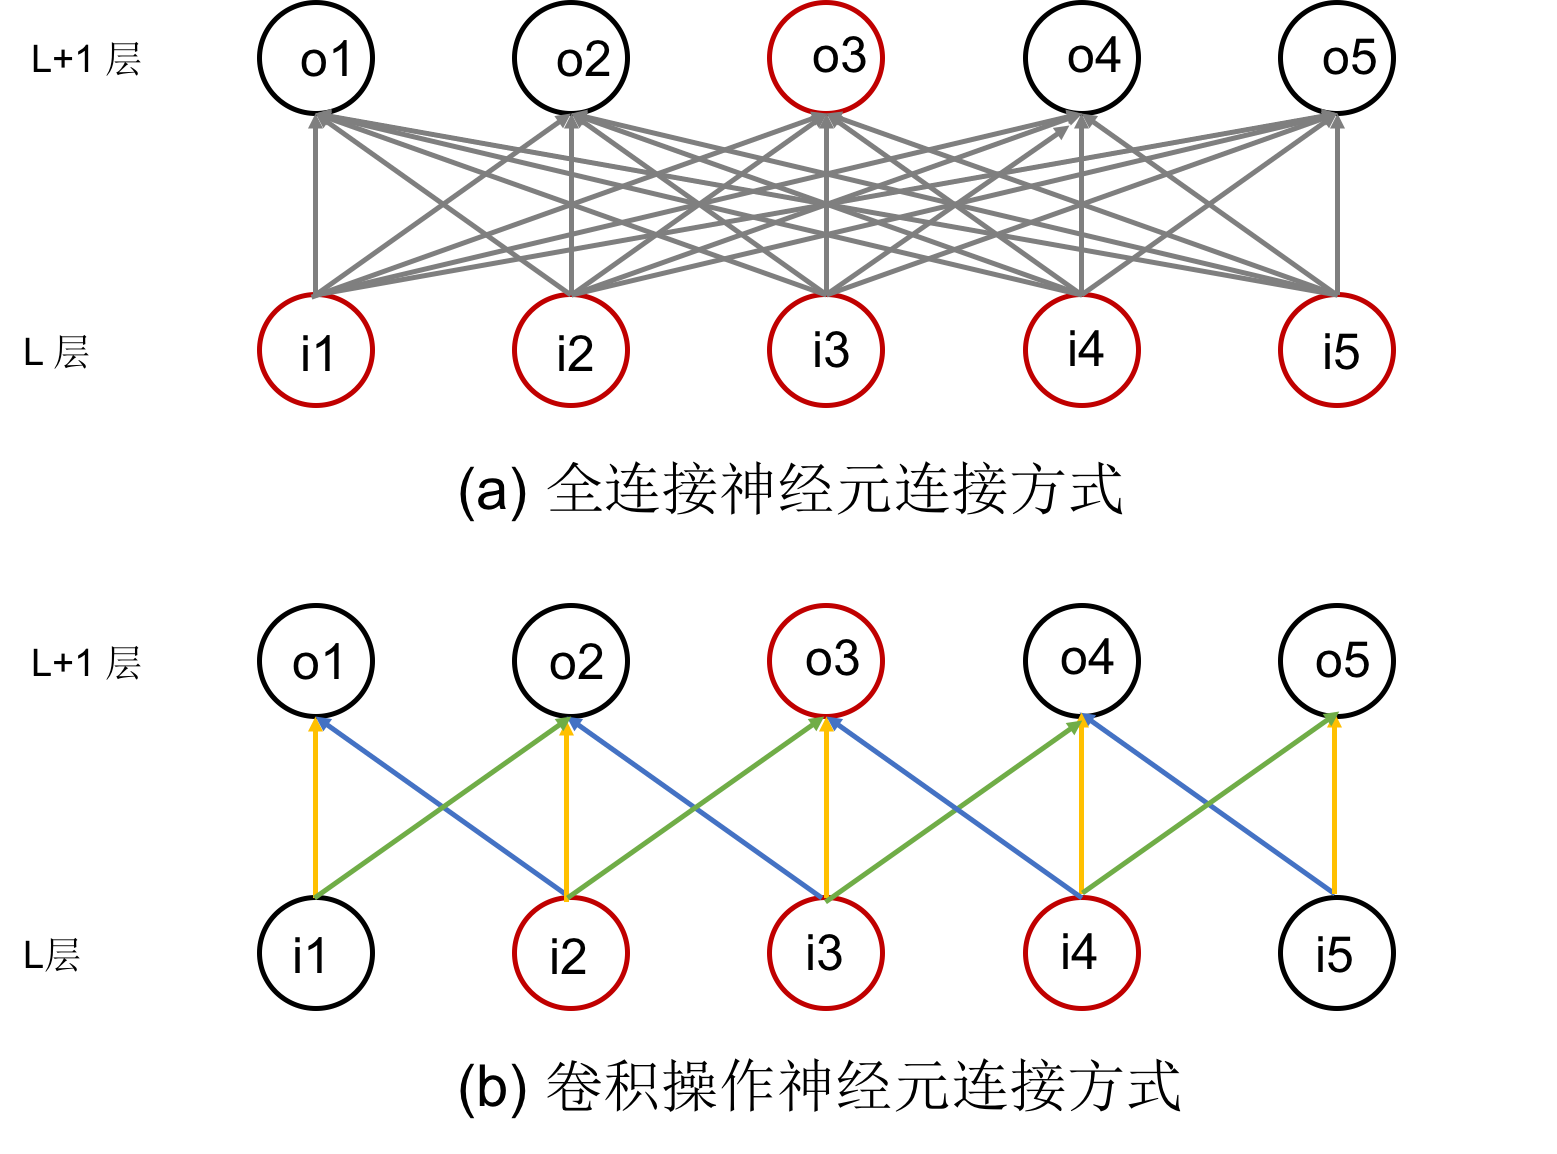
\includegraphics[width=0.8\linewidth]{intro_sparse.png}
\caption{稀疏连接与权值共享。图(a)是全连接神经元的连接方式,对于图中高亮的输出神经元o3,所有的输入神经元i1,i2,i3,i4,i5均参与了全连接运算。图(b)是卷积操作神经元的连接方式,对于高亮的输出神经元o3,与之位置相邻的三个输入神经元i2,i3,i4参与了卷积运算。即卷积操作相对于全连接具有稀疏连接的特性。卷积的权值共享,如图(b)所示,从输入到输出的连接权中,相同颜色的连线具有相同的权值参数。对于图中的例子,一共13条从输入到输出的连接权具有三种不同的颜色,即对应了三种不同的权重参数。举例来说,对于绿色的连接边,从i1到o2,从i2到o3,从i3到o4,从i4到o5,这四条边具有相同的参数,即权值共享。}
\label{fig:intro_sparse}
\end{figure}


传统的神经网络采用矩阵乘法来实现输入到输出的映射,对于每个输出单元需要所有的输入神经元参与乘法运算。卷积神经网络采用稀疏连接(稀疏权重)的方式来实现特征提取,如图~\ref{fig:intro_conv}所示,特征核的大小远远小于输入图像的大小。对于一张具有成千上万个像素点的输入图像,卷积神经网络采用十几个或上百个像素的特征核就可以有效地提取图像的局部特征,例如颜色、边缘、角点等。这意味着相对于传统的神经网络,卷积神经网络需要较少的参数,可以有效地减少模型参数,强化图像局部区域内的特征统计特性。此外,更少的卷积核参数意味着更少的乘法操作,对网络计算速度具有较大的提升。卷积稀疏连接的示例如图~\ref{fig:intro_sparse}所示,图~\ref{fig:intro_sparse}(a)是全连接神经元的连接方式,对于高亮的输出神经元o3,所有的输入神经元i1,i2,i3,i4,i5均参与了全连接运算。图~\ref{fig:intro_sparse}(b)中卷积神经元的连接方式,对于高亮的输出神经元o3,与之位置相邻的三个输入神经元i2,i3,i4参与了卷积运算。可以看出,卷积操作相对于全连接具有稀疏连接的特性。

尽管单层的卷积具有稀疏连接的特点,但是在深层的卷积神经网络结构中,卷积逐层堆叠的方式,使得深层的神经元可以间接地连接到多个输入单元,如图~\ref{fig:intro_rf}所示。如果L层代表输入图像,对于 $3\times3$ 感受野大小的卷积操作,L+1层的感受野大小为 $3\times3$,L+2层相对于L+1层具有 $3\times3$ 的感受野,但是相对于输出层L层,L+2层的感受野大小为 $5\times5$。尽管对于单层的卷积操作来说,从输入到输出神经元的连接具有稀疏的特点,但是多个卷积层的堆叠,使得深层神经元可以间接地作用于绝大部分甚至整张输入图像。这使得卷积神经网络可以通过多层卷积结构的堆叠来实现复杂的特征提取。

\begin{figure}
\centering
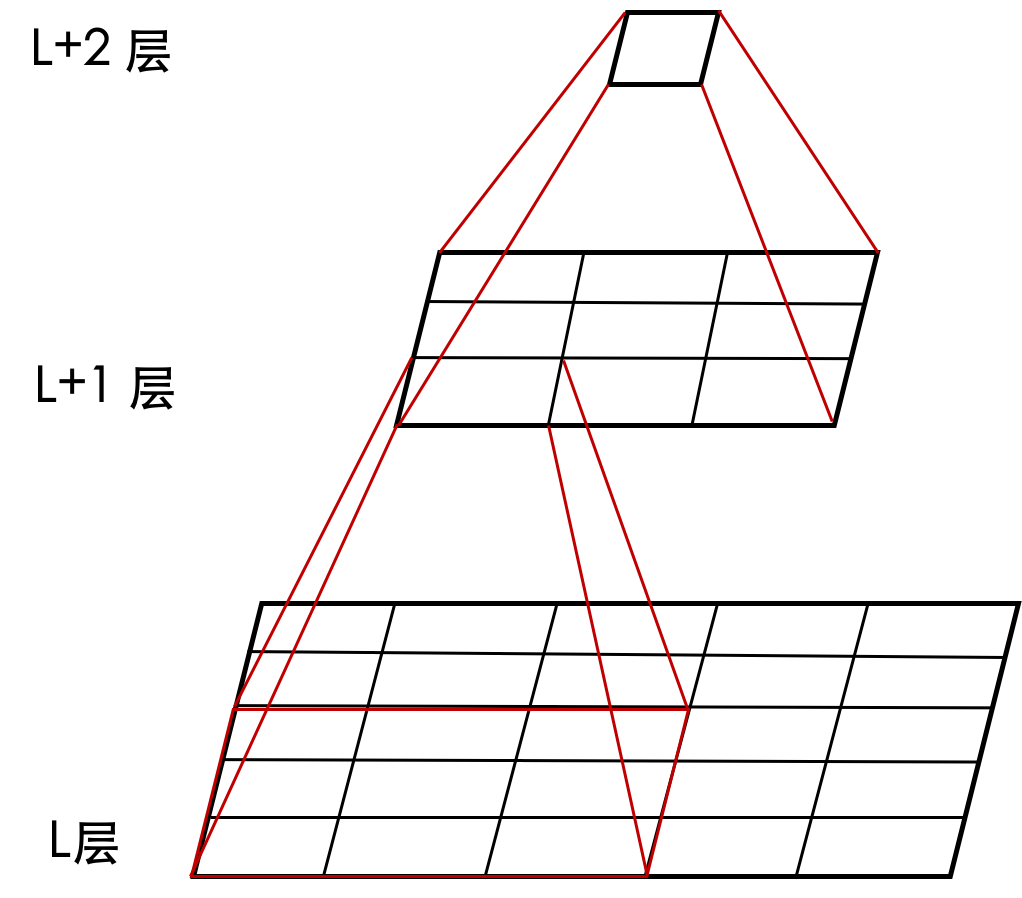
\includegraphics[width=0.7\linewidth]{intro_rf.png}
\caption{高层神经元的感受野。在深层卷积神经网络中,高层神经元的感受野范围大于浅层神经元的感受野,且随着深度的加深,感受野会逐渐增大。如图所示,如果L层代表输入图像,对于 $3\times3$ 感受野大小的卷积操作,L+1层的感受野大小为 $3\times3$,L+2层相对于L+1层具有 $3\times3$ 的感受野,但是相对于输出层L层,L+2层的感受野大小为 $5\times5$。尽管对于单层的卷积操作来说,从输入到输出神经元的连接具有稀疏的特点,但是多个卷积层的堆叠,使得深层神经元可以间接地作用于绝大部分甚至整张输入图像。}
\label{fig:intro_rf}
\end{figure}

参数共享是指在卷积神经网络中复用了某些参数。在传统的神经网络中,权重矩阵的每一个元素只使用一次,每个权重参数只和对应位置的一个输入相乘。权值共享的一个另一种表示是权重捆绑(Tied Weights),即某个位置的一组权重与其他位置的权重捆绑在一起,具有相同的参数。在卷积神经网络中,不同位置的卷积核共享同一组参数。参数共享并没有影响网络的前向传播时间,但是可以有效地较少模型的参数。一维空间的权值共享如图~\ref{fig:intro_sparse}(b)所示。对于图~\ref{fig:intro_sparse}(b)中的例子,一共13条从输入到输出的连接权具有三种不同的颜色,即对应了三种不同的权重参数。举例来说,对于绿色的连接边,从i1到o2,从i2到o3,从i3到o4,从i4到o5,这四条边具有相同的参数,即权值共享。

\begin{figure}
\centering
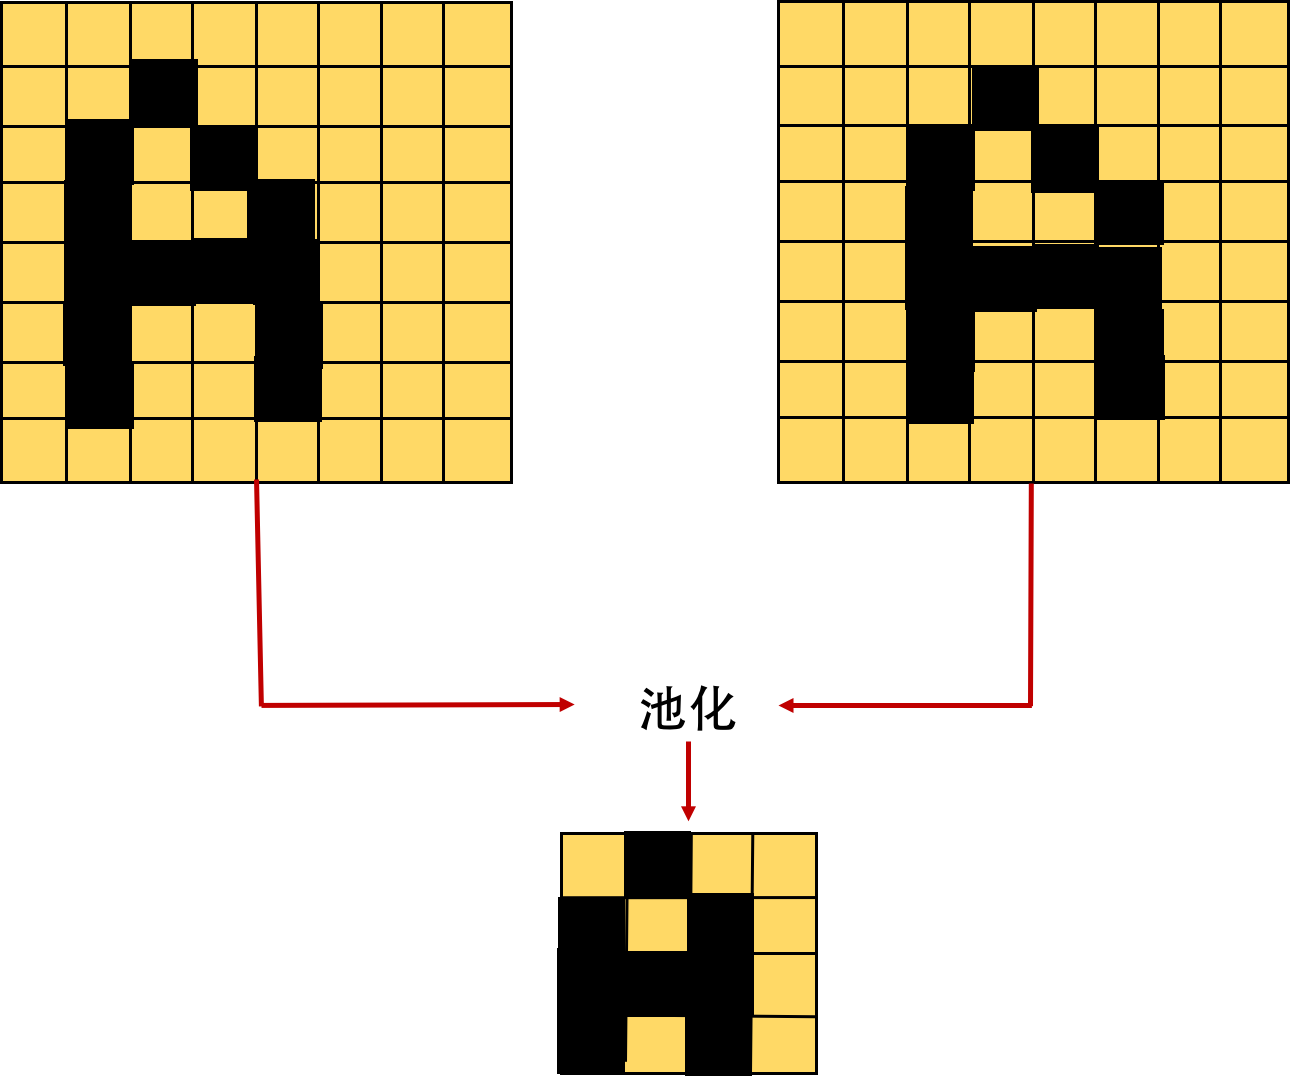
\includegraphics[width=1\linewidth]{intro_pooling.png}
\caption{池化操作的平移不变性。右图中的字母A相对于左图的A具有一个较为微小的平移,但是通过最大池化操作,却得到了完全相同的输出结果。即池化操作具有一定的特征不变性。}
\label{fig:intro_pooling}
\end{figure}

卷积神经网络中,参数共享的性质使卷积具有了平移同变性。一个函数具有同变性是指,输出与输入具有相同的变化。对于图像卷积操作,通常会生成一个二维特征图,其中包含了输入图像中物体的位置信息。如果输入图像中的物体有所移动,经过相同的卷积操作,输出特征图中物体的特征也会进行同尺度的移动。平移同变性使我们可以采用卷积操作提取图像的局部特征,例如图像处理过程中,提取图像的边缘特征是浅层网络的一个必要且有效的操作。而图像的边缘特征往往分布于整张图像的多处位置,因此在整张图像上采用权值共享是一个实际有效且十分可行的方案。但是在某些情况下,我们也许不希望采用参数共享,例如在人脸识别任务中,我们也许希望在人脸的不同位置提取不同的特征,例如在图像的上半部分提取眉毛特征,而在图像的下半部分查找出下巴等信息。卷积操作对平移具有同变性,但是对于缩放或旋转等变换并不具备同变性,需要卷积神经网络的其他机制去处理缩放和旋转问题。


池化操作可以理解为局部区域内相邻特征的统计输出,例如最大池化的输出是相邻矩形区域内特征的最大值,而均值池化的输出是相邻区域内特征的平均值。池化使特征具有一定程度的平移不变性,也就是说如果我们将输入图像上的物体进行小幅度的平移,池化的输出结果与平移前相同,如图~\ref{fig:intro_pooling}所示。图~\ref{fig:intro_pooling}中对一个具有微小平移的两幅输入图像,均采用最大池化进行特征提取,最终得到完全相同的输出结果。对于一些位置无关的图像识别任务,平移不变性是一个特征提取的有效手段。池化操作相当于我们给待处理的问题引入了平移不变性的先验知识,如果待处理的问题确实具有这样的性质,可以极大地提高网络的特征提取能力。

\begin{figure}
\centering
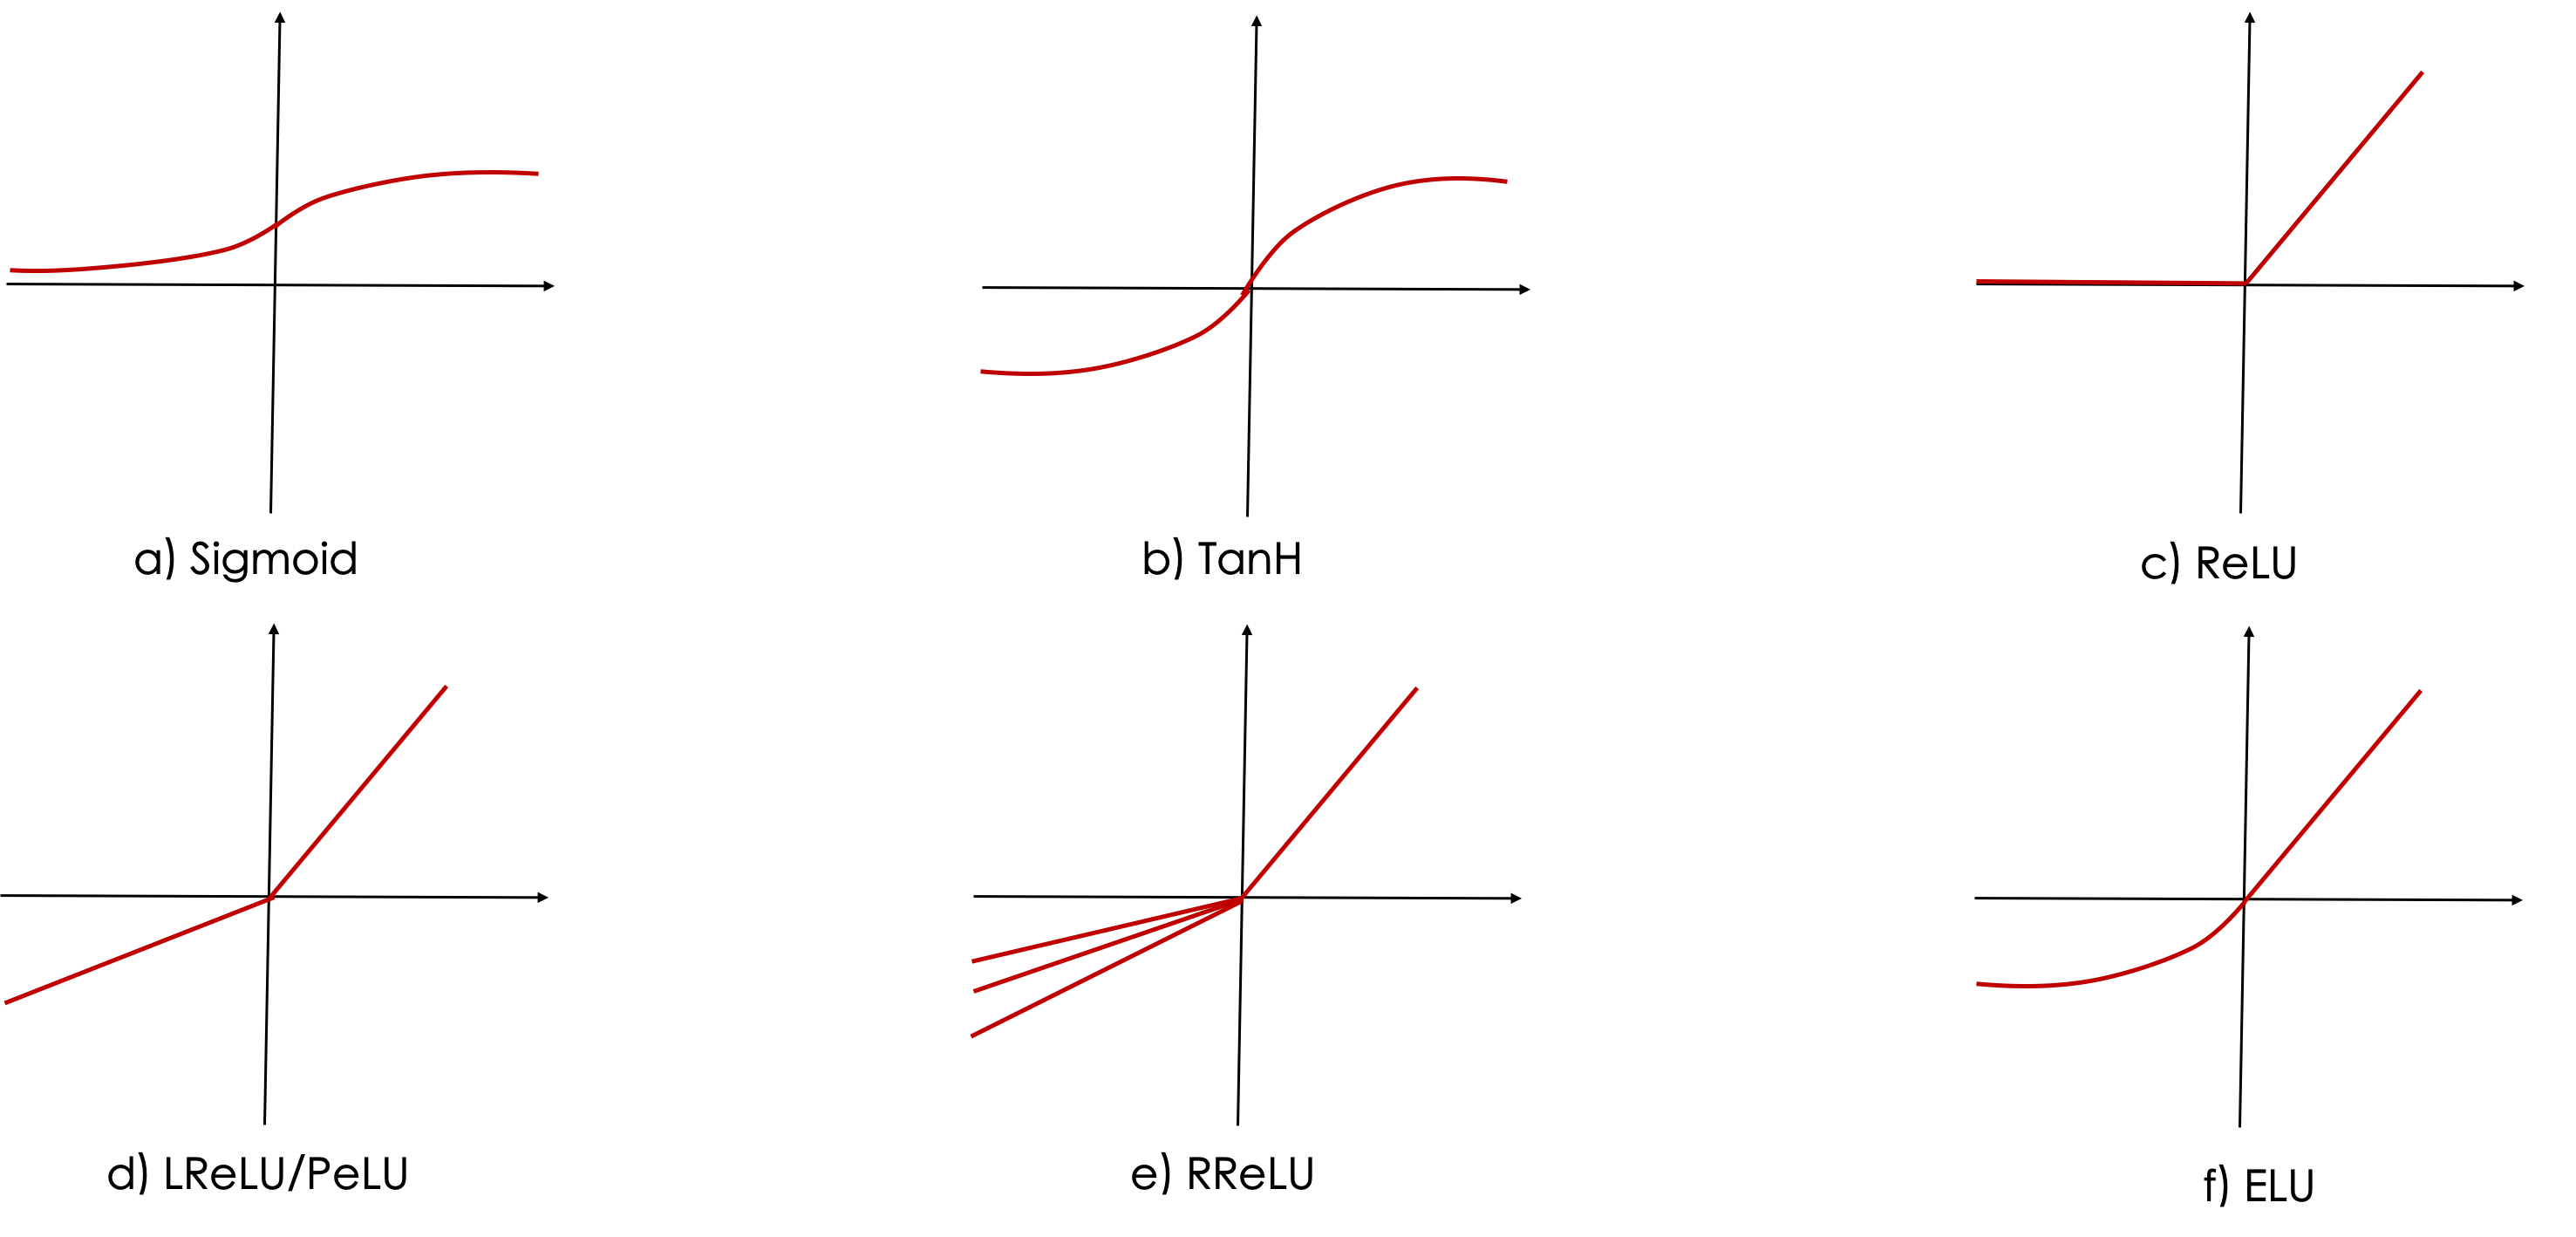
\includegraphics[width=1\linewidth]{intro_active.png}
\caption{不同激活函数的函数曲线对比图。}
\label{fig:intro_active}
\end{figure}

非线性激活函数可以增强卷积神经网络的非线性拟合能力,不同形式的激活函数,对网络的计算量、特征的非线性拟合能力和网络的泛化能力具有重要的影响。ReLU~\cite{nair2010rectified}是目前卷积神经网络最常用的激活函数,它是一个作用于单像素的线性分段函数,ReLU保留正数输入不变同时将负的输入抑制为零,其函数形式可以表示为:
\begin{eqnarray} \label{equ:relu}
h_{i,j,k}=\max(x_{i,j,k},0)
\end{eqnarray}
其中$x_{i,j,k}$表示第 $k$ 个通道位置 $(i,j)$ 处的输入特征。相对于传统的Sigmoid函数:
\begin{eqnarray} \label{equ:sigmoid}
h_{i,j,k}=\frac{1}{1+e^{-x_{i,j,k}}}
\end{eqnarray}
和双曲正切函数:
\begin{eqnarray} \label{equ:tanh}
h_{i,j,k}=\frac{e^{x_{i,j,k}}-e^{-x_{i,j,k}}}{e^{x_{i,j,k}}+e^{-x_{i,j,k}}}
\end{eqnarray}
ReLU的计算更简单,并且在输出神经元中引入稀疏的概念,可以得到稀疏的特征表达。但是对于未激活的神经元,ReLU的反向传播梯度为零,使得未激活的神经元无法进行参数更新。Mass等人~\cite{maas2013rectifier}提出斜坡线性整流单元(Leaky Rectified linear unit,LReLU)来解决这个问题,计算公式如下:
\begin{eqnarray} \label{equ:lrelu}
h_{i,j,k}=\max(x_{i,j,k},0)+{\lambda}\min(x_{i,j,k},0)
\end{eqnarray}
其中$\lambda$是一个预定义的取值在 $(0,1)$ 之间的随机变量。He等人~\cite{he2015delving}对LReLU进一步改进,提出了参数化线性整流单元(Parametric Rectified linear unit,PReLU),PReLU可以表示为:
\begin{eqnarray} \label{equ:prelu}
h_{i,j,k}=\max(x_{i,j,k},0)+{\lambda}_k\min(x_{i,j,k},0)
\end{eqnarray}
其中 ${\lambda}_k$ 是第 $k$ 个通道上的可学习参数。PReLU通过引入极少的参数,有效地提高了特征的拟合能力。对LReLU的另一项改进是Xu等人~\cite{xu2015empirical}提出的随机线性整流单元(Randomized Rectified linear unit,RReLU),与公式~\ref{equ:prelu}具有相同的形式,但是其中的 ${\lambda}_k$ 服从均匀分布,前向传播过程中通过随机采样产生。Clevert等人~\cite{clevert2015fast}提出了指数线性单元(Exponential Linear Unit,ELU),对激活函数的负数部分进入饱和机制,可以有效加快网络的收敛速度,ELU可以表示为:
\begin{eqnarray} \label{equ:elu}
h_{i,j,k}=\max(x_{i,j,k},0)+\min({\lambda}(e^{z_{i,j,k}}-1),0)
\end{eqnarray}
其中 $\lambda$ 是一个预定义的加权因子。上述六种非线性激活函数的关系与对比如图~\ref{fig:intro_active}所示。


\section{问题提出}
\label{sec:question}

卷积神经网络凭借局部感受野、权值共享、池化和分层特征提取四大特点,在计算机视觉领领域,别是视觉物体识别任务上取得了重大的研究突破。自2012年Krizhevsky等人~\cite{krizhevsky2012imagenet}在ImageNet大规模视觉识别比赛夺冠之后,各种卷积网络模型如ZFNet~\cite{zeiler2014visualizing},VGG~\cite{simonyan2014very},GoogLeNet~\cite{szegedy2014going,szegedy2015rethinking,szegedy2016inception}、ResNet~\cite{he2015deep}等被相继提出,用以解决物体识别问题。

但是对于一个新的物体识别问题,针对具体任务设计并实现一个有效的网络模型仍然是一个困难的工作,网络深度的选择、感受野大小的选择和卷积核个数的选择都是网络在设计过程中普遍存在却又很难回答的问题。例如在深度选择上,VGG和GoogLeNet的成功说明了更深的网络结构可以提高网络的识别率,但是另一方面ResNet通过实验证实,随着网络的深度逐渐加深,网络的识别性能将趋于饱和甚至下降。尽管卷积神经网络具有卷积、池化和非线性化等通用的结构,但是整个网络的设计过程仍然是经验主义的。另一方面,在物体识别任务上,已经出现了很多结构功能各不相同的卷积神经网络模型,并且这些模型在各自不同的领域均得到了验证。对这些模型进行总结、归纳和积累,综合他们各自的优势,用于解决新的识别问题,这也是一个具有研究意义的课题。因此,本文提出了一种组合卷积结构,即自适应卷积模块,来简化复杂网络的设计过程。在组合卷积结构中,融合了四种网络模型的特点与优势,用以提高组合卷积结构的特征表达能力。

对于视觉物体识别任务,网络的泛化能力是一个重要的评价指标。卷积神经网络能够在物体识别任务上取得成功的一个关键因素就是大规模的标注数据,当我们无法获取更多的标注数据时,数据增广是一个直接有效的提高网络识别能力和泛化能力的方法。合理的数据增广方式,可以在不影响样本总体分布的前提下,扩充样本空间,增加输入图像的多样性。但是卷积神经网络采用分层的特征提取方式,并且特征在逐层提取的过程中会不断强化其旋转平移的不变性,因此从输入层到输出层,数据增广对网络的参数更新的影响会逐渐减弱。本文将数据增广的思想扩展到特征层,提出了随机区域池化方法,对池化层特征进行特征增广,在不改变特征空间样本分布的前提下,对特征进行扰动,增加特征的多样性。通过特征增广来增强网络的鲁棒性,提高网络的泛化能力。

卷积神经网络优越的识别能力往往来自于更深或更宽的网络结构和更大的计算规模。具有大量参数的卷积神经网络模型,在测试或预测阶段需要消耗大量的计算资源与时间,很难在实际生活中得到大规模的应用与推广。因为需要消耗大量的内存和计算资源,因此无法将应用部署于客户端;部署在高性能服务器,服务端也无法应对多用户的并发请求;就算只对单用户提供服务,用户端也无法接受很长的结果查询响应时间。为了解决卷积神经网络应用与部署的难题,早期的工作主要集中在硬件性能的提升,但硬件方面的研究进展已经无法满足人们对计算能力的需求,特别是在当今这样一个移动互联网时代,智能手机和平板电脑成为人们生活的主流产品,如何在一个低性能的CPU和只具有少量内存的GPU上运行深度卷积神经网络模型,逐渐引起学术界的关注。本文提出了一种新的基于矩阵低秩分解的卷积压缩方法主导卷积核分解,用于对卷积神经网络模型进行参数压缩与模型提速,并提出知识预回归的训练方法来尽力弥补由模型压缩所引起的精度损失。


\section{主要研究贡献}

针对上文提到的问题,本文对卷积神经网络进行了研究与改进,主要研究贡献包括:

提出了一种组合卷积结构:自适应卷积模块,用于简化复杂卷积神经网络的设计过程。通过对组合卷积模块的简单堆叠,来实现通用网络结构的设计。组合卷积结构结合了盗梦空间网络Inception、最大化输出单元Maxout、残差网络ResNet和网络中的网络NIN四个模型的优点,使得组合卷积结构具有更强的特征提取能力和更快的网络收敛速度。

提出了池化的一种改进方法:随机区域池化,将数据增广的思想从数据层扩展到特征层,对卷积神经网络池化层特征进行特征增广。随机区域池化采用随机仿射变换对池化区域进行重采样,再对重采样之后的区域进行池化操作,因仿射变换后的池化区域往往处于非整数边界,因此双线性差值被用于对非整数边界的特征进行估计。随机区域池化可以有效地增加特征的多样性,使网络对特征的扰动更加鲁棒,从而提高网络的泛化能力。

提出了一种基于主导卷积核分解和知识预回归的参数压缩与网络加速方法。主导卷积核分解是一种受矩阵低秩分解启发的卷积参数压缩方法,通过保留一个或多个具有主导作用的卷积核对卷积参数进行压缩。主导卷积核分解可以将卷积层的参数和计算量压缩到接近原来的12\%,极大地提高了模型的预测速度。为了弥补网络因参数压缩所造成的精度损失,受知识蒸馏方法启发,我们提出了知识预回归的网络训练方法,让压缩后的网络可以逐层地学习原网络的特征表达和泛化能力。

针对交通标志识别任务,我们将组合卷积结构和随机区域池化相结合,验证了两个方法的有效性。并采用主导卷积核分解对模型进行压缩,最后通过知识预回归训练方法提高模型的泛化能力,最终得到一个适用于交通标志识别的高精度快速卷积神经网络模型。

\section{章节安排}


\begin{figure}[h]
\centering
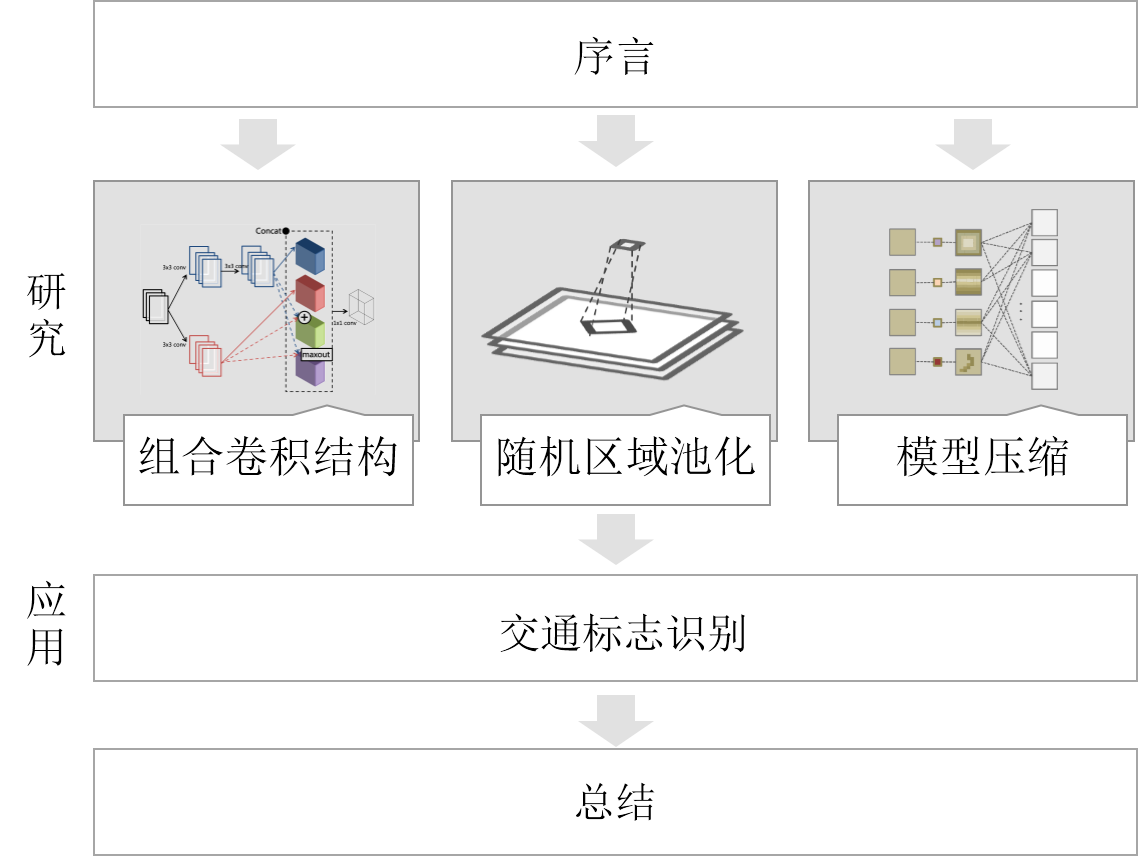
\includegraphics[width=0.8\linewidth]{intro_arc.png}
\caption{各章节关系图。}
\label{fig:intro_arc}
\end{figure}

本文共分为六章,各章之间的联系如图~\ref{fig:intro_arc}所示,具体内容安排如下:

第一章为绪论,介绍了本文的研究背景与意义,调研了卷积神经网络近年来的发展现状,总结了在物体识别任务中卷积神经网络存在的问题,针对这些问题提出了本文的研究内容。

第二章为了简化复杂卷积卷积神经网络的设计过程,提出了一种组合卷积结构:自适应卷积模块。本章详细介绍了组合卷积结构的实现细节,并以物体识别任务为例进行了实验验证与分析。

第三章为了提高网络的泛化能力,提出了池化层的一种改进方法随机区域池化。该章详细阐述了随机区域池化的思想与实现,同样以物体识别任务为例验证了随机区域池化的泛化能力。

第四章针对卷积神经网络的部署与应用的难题,提出了基于主导卷积核分解和知识预回归的参数压缩与网络加速方法。详细分析了主导卷积核的参数压缩方法和为了提高网络泛化能力的知识预回归训练方法。

第五章针对一个实际问题:交通标志识别,对第二章的组合卷积结构和第三章的随机区域池化进行了实验验证与对比分析。之后将两种方法结合,应用于交通标志识别任务。最终采用第四章的模型压缩方法对网络进行加速,得到一个适用于交通标志识别的高精度快速模型。

第六章是对全文工作的总结,并展望了未来可能的研究方向。

